\documentclass[twoside]{book}

% Packages required by doxygen
\usepackage{fixltx2e}
\usepackage{calc}
\usepackage{doxygen}
\usepackage[export]{adjustbox} % also loads graphicx
\usepackage{graphicx}
\usepackage[utf8]{inputenc}
\usepackage{makeidx}
\usepackage{multicol}
\usepackage{multirow}
\PassOptionsToPackage{warn}{textcomp}
\usepackage{textcomp}
\usepackage[nointegrals]{wasysym}
\usepackage[table]{xcolor}

% Font selection
\usepackage[T1]{fontenc}
\usepackage[scaled=.90]{helvet}
\usepackage{courier}
\usepackage{amssymb}
\usepackage{sectsty}
\renewcommand{\familydefault}{\sfdefault}
\allsectionsfont{%
  \fontseries{bc}\selectfont%
  \color{darkgray}%
}
\renewcommand{\DoxyLabelFont}{%
  \fontseries{bc}\selectfont%
  \color{darkgray}%
}
\newcommand{\+}{\discretionary{\mbox{\scriptsize$\hookleftarrow$}}{}{}}

% Page & text layout
\usepackage{geometry}
\geometry{%
  a4paper,%
  top=2.5cm,%
  bottom=2.5cm,%
  left=2.5cm,%
  right=2.5cm%
}
\tolerance=750
\hfuzz=15pt
\hbadness=750
\setlength{\emergencystretch}{15pt}
\setlength{\parindent}{0cm}
\setlength{\parskip}{3ex plus 2ex minus 2ex}
\makeatletter
\renewcommand{\paragraph}{%
  \@startsection{paragraph}{4}{0ex}{-1.0ex}{1.0ex}{%
    \normalfont\normalsize\bfseries\SS@parafont%
  }%
}
\renewcommand{\subparagraph}{%
  \@startsection{subparagraph}{5}{0ex}{-1.0ex}{1.0ex}{%
    \normalfont\normalsize\bfseries\SS@subparafont%
  }%
}
\makeatother

% Headers & footers
\usepackage{fancyhdr}
\pagestyle{fancyplain}
\fancyhead[LE]{\fancyplain{}{\bfseries\thepage}}
\fancyhead[CE]{\fancyplain{}{}}
\fancyhead[RE]{\fancyplain{}{\bfseries\leftmark}}
\fancyhead[LO]{\fancyplain{}{\bfseries\rightmark}}
\fancyhead[CO]{\fancyplain{}{}}
\fancyhead[RO]{\fancyplain{}{\bfseries\thepage}}
\fancyfoot[LE]{\fancyplain{}{}}
\fancyfoot[CE]{\fancyplain{}{}}
\fancyfoot[RE]{\fancyplain{}{\bfseries\scriptsize Generated by Doxygen }}
\fancyfoot[LO]{\fancyplain{}{\bfseries\scriptsize Generated by Doxygen }}
\fancyfoot[CO]{\fancyplain{}{}}
\fancyfoot[RO]{\fancyplain{}{}}
\renewcommand{\footrulewidth}{0.4pt}
\renewcommand{\chaptermark}[1]{%
  \markboth{#1}{}%
}
\renewcommand{\sectionmark}[1]{%
  \markright{\thesection\ #1}%
}

% Indices & bibliography
\usepackage{natbib}
\usepackage[titles]{tocloft}
\setcounter{tocdepth}{3}
\setcounter{secnumdepth}{5}
\makeindex

% Hyperlinks (required, but should be loaded last)
\usepackage{ifpdf}
\ifpdf
  \usepackage[pdftex,pagebackref=true]{hyperref}
\else
  \usepackage[ps2pdf,pagebackref=true]{hyperref}
\fi
\hypersetup{%
  colorlinks=true,%
  linkcolor=blue,%
  citecolor=blue,%
  unicode%
}

% Custom commands
\newcommand{\clearemptydoublepage}{%
  \newpage{\pagestyle{empty}\cleardoublepage}%
}

\usepackage{caption}
\captionsetup{labelsep=space,justification=centering,font={bf},singlelinecheck=off,skip=4pt,position=top}

%===== C O N T E N T S =====

\begin{document}

% Titlepage & ToC
\hypersetup{pageanchor=false,
             bookmarksnumbered=true,
             pdfencoding=unicode
            }
\pagenumbering{alph}
\begin{titlepage}
\vspace*{7cm}
\begin{center}%
{\Large P2P \\[1ex]\large 1 }\\
\vspace*{1cm}
{\large Generated by Doxygen 1.8.13}\\
\end{center}
\end{titlepage}
\clearemptydoublepage
\pagenumbering{roman}
\tableofcontents
\clearemptydoublepage
\pagenumbering{arabic}
\hypersetup{pageanchor=true}

%--- Begin generated contents ---
\chapter{p2p\+\_\+stri}
\label{index}\hypertarget{index}{}This Java project is developped in collaboration with Romain B\+R\+E\+D\+A\+R\+I\+OL \& Léo-\/\+Paul Dewitte.

\doxysection*{Goal}

This application act as a P2P Client to share files.

\doxysection*{Subject}

{\bfseries{But}} \+: le but de ce projet est de créer une application répartie en Java de téléchargement de fichier en mode P2P (peer to peer ou poste à poste). Les étapes suivantes sont conseillées. \doxysubsection*{Étape 1 \+: Téléchargement à la F\+TP}

La première étape doit permettre de télécharger un fichier en intégralité d\textquotesingle{}une machine vers une autre machine de façon similaire aux applications suivant le protocole F\+TP.

Plan de travail \+:


\begin{DoxyItemize}
\item Lire le sujet jusqu\textquotesingle{}au bout et la R\+FC F\+TP (version anglaise, version française)
\item Concevoir l\textquotesingle{}application répartie avec U\+ML
\item Écrire l\textquotesingle{}application serveur et l\textquotesingle{}application cliente.
\end{DoxyItemize}

\doxysubsection*{Étape 2 \+: Téléchargement en parallèle}

Dans la seconde étape, on permet à un client de télécharger le fichier depuis plusieurs serveurs. Le fichier sera découpé en plusieurs blocs de tailles égales (par exemple 4 Ko) qui seront téléchargés depuis plusieurs serveurs. Dans cette étape c\textquotesingle{}est le client qui choisit (par exemple aléatoirement) quel bloc télécharger depuis quel serveur.

Plan de travail \+:


\begin{DoxyItemize}
\item Modifier le serveur pour gérer l\textquotesingle{}envoi de n\textquotesingle{}importe quel bloc d\textquotesingle{}un fichier
\item Modifier le client pour qu\textquotesingle{}il puisse demander le téléchargement de n\textquotesingle{}importe quel bloc et re-\/créer le fichier complet.
\end{DoxyItemize}

\doxysubsection*{Étape 3 \+: Transformation en P2P simple}

Dans cette étape, il n\textquotesingle{}y a plus de clients ni de serveurs ; les applications sont les deux à la fois. Chaque application devra noter de quelle partie du fichier elle dispose. Au démarrage certaines applications auront le fichier complet et les autres aucun bloc. Les applications demanderont aléatoirement chaque bloc manquant à n\textquotesingle{}importe quelle autre application qui renverra soit le bloc soit un message d\textquotesingle{}erreur.

\doxysubsection*{Étape 4 \+: P2P coordonné}

Dans cette étape, on ajoute un serveur dont le rôle est de maintenir la liste des applications gérant le téléchargement d\textquotesingle{}un fichier et quel bloc chaque application possède. Ce serveur coordonnera le téléchargement en précisant à chaque application, à qui se connecter et ce qui y est disponible.

\doxysubsection*{Étape 5 \+: P2P coopératif}

Dans cette étape, on doit s\textquotesingle{}assurer que les applications envoient et reçoivent globalement les même quantités. On essaiera ainsi de désavantager les applications qui ne font que télécharger et n\textquotesingle{}envoient rien.

\doxysubsection*{Options \+:}


\begin{DoxyItemize}
\item Créer une I\+HM (interface homme machine) Graphique pour les applications avec Swing par exemple.
\item Gérer à la fois des communications U\+DP et T\+CP. 
\end{DoxyItemize}
\chapter{Hierarchical Index}
\section{Class Hierarchy}
This inheritance list is sorted roughly, but not completely, alphabetically\+:\begin{DoxyCompactList}
\item \contentsline{section}{terminal\+Client.\+Gestionnaire\+Fichier}{\pageref{classterminalClient_1_1GestionnaireFichier}}{}
\item \contentsline{section}{central\+Server.\+Liste\+Des\+Fichiers\+Complets}{\pageref{classcentralServer_1_1ListeDesFichiersComplets}}{}
\item \contentsline{section}{central\+Server.\+Liste\+Des\+Info\+Utilisateur}{\pageref{classcentralServer_1_1ListeDesInfoUtilisateur}}{}
\item \contentsline{section}{commun.\+Messages}{\pageref{classcommun_1_1Messages}}{}
\item Runnable\begin{DoxyCompactList}
\item \contentsline{section}{gestionnaire\+Requete.\+Gestionnaire\+Requetes}{\pageref{classgestionnaireRequete_1_1GestionnaireRequetes}}{}
\begin{DoxyCompactList}
\item \contentsline{section}{gestionnaire\+Requete.\+Gestionnaire\+Requetes\+Serveur}{\pageref{classgestionnaireRequete_1_1GestionnaireRequetesServeur}}{}
\item \contentsline{section}{gestionnaire\+Requete.\+Gestionnaire\+Requetes\+Serveur\+Central}{\pageref{classgestionnaireRequete_1_1GestionnaireRequetesServeurCentral}}{}
\end{DoxyCompactList}
\item \contentsline{section}{requete.\+Requete}{\pageref{classrequete_1_1Requete}}{}
\begin{DoxyCompactList}
\item \contentsline{section}{gestionnaire\+Requete.\+Gestionnaire\+De\+Telechargement}{\pageref{classgestionnaireRequete_1_1GestionnaireDeTelechargement}}{}
\item \contentsline{section}{requete.\+Requete\+Liste}{\pageref{classrequete_1_1RequeteListe}}{}
\item \contentsline{section}{requete.\+Requete\+Telecharger}{\pageref{classrequete_1_1RequeteTelecharger}}{}
\item \contentsline{section}{requete.\+Requete\+Update\+Infos\+Utilisateur}{\pageref{classrequete_1_1RequeteUpdateInfosUtilisateur}}{}
\end{DoxyCompactList}
\item \contentsline{section}{terminal\+Client.\+Gestionnaire\+Infos\+Utilisateur}{\pageref{classterminalClient_1_1GestionnaireInfosUtilisateur}}{}
\item \contentsline{section}{terminal\+Client.\+Serveur}{\pageref{classterminalClient_1_1Serveur}}{}
\end{DoxyCompactList}
\item \contentsline{section}{central\+Server.\+Serveur\+Central}{\pageref{classcentralServer_1_1ServeurCentral}}{}
\item \contentsline{section}{central\+Server.\+Serveur\+Central\+Main}{\pageref{classcentralServer_1_1ServeurCentralMain}}{}
\item \contentsline{section}{terminal\+Client.\+Terminal\+Main}{\pageref{classterminalClient_1_1TerminalMain}}{}
\item Serializable\begin{DoxyCompactList}
\item \contentsline{section}{commun.\+Info\+Utilisateur}{\pageref{classcommun_1_1InfoUtilisateur}}{}
\item \contentsline{section}{commun.\+Liste\+De\+Blocs}{\pageref{classcommun_1_1ListeDeBlocs}}{}
\end{DoxyCompactList}
\end{DoxyCompactList}

\chapter{Class Index}
\section{Class List}
Here are the classes, structs, unions and interfaces with brief descriptions\+:\begin{DoxyCompactList}
\item\contentsline{section}{\hyperlink{classclient_1_1Client}{client.\+Client} }{\pageref{classclient_1_1Client}}{}
\item\contentsline{section}{\hyperlink{classcommon_1_1Messages}{common.\+Messages} }{\pageref{classcommon_1_1Messages}}{}
\item\contentsline{section}{\hyperlink{classserveur_1_1Serveur}{serveur.\+Serveur} }{\pageref{classserveur_1_1Serveur}}{}
\item\contentsline{section}{\hyperlink{classcommon_1_1Socket}{common.\+Socket} \\*Cette classe permet de gérer les sockets }{\pageref{classcommon_1_1Socket}}{}
\end{DoxyCompactList}

\chapter{Class Documentation}
\hypertarget{classgestionnaireRequete_1_1GestionnaireDeTelechargement}{}\section{gestionnaire\+Requete.\+Gestionnaire\+De\+Telechargement Class Reference}
\label{classgestionnaireRequete_1_1GestionnaireDeTelechargement}\index{gestionnaire\+Requete.\+Gestionnaire\+De\+Telechargement@{gestionnaire\+Requete.\+Gestionnaire\+De\+Telechargement}}


cette classe va gérer les téléchargements d\textquotesingle{}un fichier depuis un ou plusieurs autres clients.  




Inheritance diagram for gestionnaire\+Requete.\+Gestionnaire\+De\+Telechargement\+:\nopagebreak
\begin{figure}[H]
\begin{center}
\leavevmode
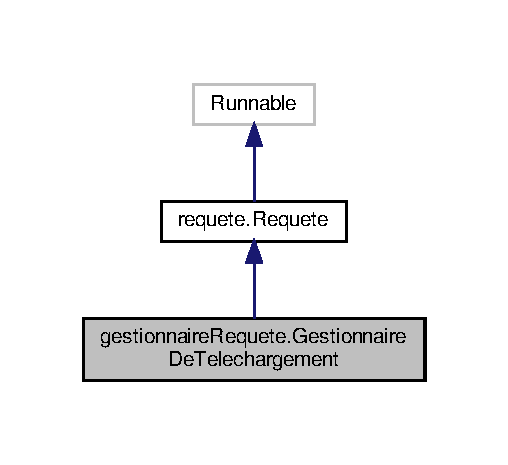
\includegraphics[width=244pt]{classgestionnaireRequete_1_1GestionnaireDeTelechargement__inherit__graph}
\end{center}
\end{figure}


Collaboration diagram for gestionnaire\+Requete.\+Gestionnaire\+De\+Telechargement\+:\nopagebreak
\begin{figure}[H]
\begin{center}
\leavevmode
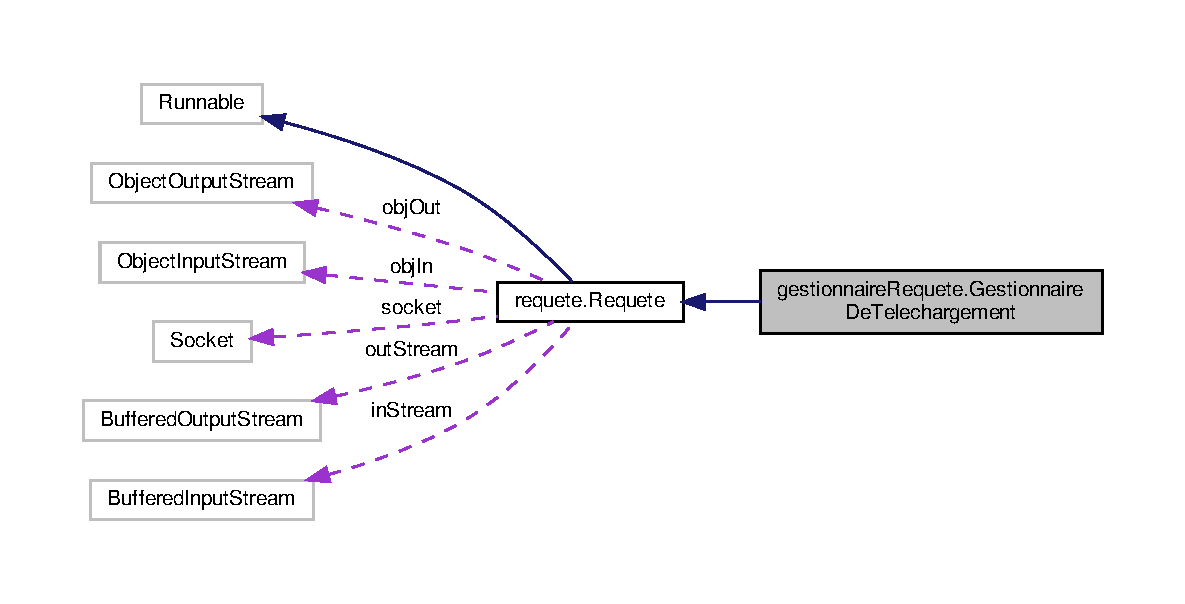
\includegraphics[width=350pt]{classgestionnaireRequete_1_1GestionnaireDeTelechargement__coll__graph}
\end{center}
\end{figure}
\subsection*{Public Member Functions}
\begin{DoxyCompactItemize}
\item 
\hyperlink{classgestionnaireRequete_1_1GestionnaireDeTelechargement_a254be2581dcadd4e17265b9460d4b229}{Gestionnaire\+De\+Telechargement} (String adresse\+Serveur\+Central, String nom\+Fichier, \hyperlink{classterminalClient_1_1GestionnaireFichier}{Gestionnaire\+Fichier} gestionnaire\+Fichier)
\begin{DoxyCompactList}\small\item\em constructeur de la classe. \end{DoxyCompactList}\item 
\mbox{\Hypertarget{classgestionnaireRequete_1_1GestionnaireDeTelechargement_ad501981a3f10e907c9466042ce2bc72f}\label{classgestionnaireRequete_1_1GestionnaireDeTelechargement_ad501981a3f10e907c9466042ce2bc72f}} 
void \hyperlink{classgestionnaireRequete_1_1GestionnaireDeTelechargement_ad501981a3f10e907c9466042ce2bc72f}{run} ()
\begin{DoxyCompactList}\small\item\em methode pour lancer le Thread. \end{DoxyCompactList}\end{DoxyCompactItemize}
\subsection*{Additional Inherited Members}


\subsection{Detailed Description}
cette classe va gérer les téléchargements d\textquotesingle{}un fichier depuis un ou plusieurs autres clients. 

\subsection{Constructor \& Destructor Documentation}
\mbox{\Hypertarget{classgestionnaireRequete_1_1GestionnaireDeTelechargement_a254be2581dcadd4e17265b9460d4b229}\label{classgestionnaireRequete_1_1GestionnaireDeTelechargement_a254be2581dcadd4e17265b9460d4b229}} 
\index{gestionnaire\+Requete\+::\+Gestionnaire\+De\+Telechargement@{gestionnaire\+Requete\+::\+Gestionnaire\+De\+Telechargement}!Gestionnaire\+De\+Telechargement@{Gestionnaire\+De\+Telechargement}}
\index{Gestionnaire\+De\+Telechargement@{Gestionnaire\+De\+Telechargement}!gestionnaire\+Requete\+::\+Gestionnaire\+De\+Telechargement@{gestionnaire\+Requete\+::\+Gestionnaire\+De\+Telechargement}}
\subsubsection{\texorpdfstring{Gestionnaire\+De\+Telechargement()}{GestionnaireDeTelechargement()}}
{\footnotesize\ttfamily gestionnaire\+Requete.\+Gestionnaire\+De\+Telechargement.\+Gestionnaire\+De\+Telechargement (\begin{DoxyParamCaption}\item[{String}]{adresse\+Serveur\+Central,  }\item[{String}]{nom\+Fichier,  }\item[{\hyperlink{classterminalClient_1_1GestionnaireFichier}{Gestionnaire\+Fichier}}]{gestionnaire\+Fichier }\end{DoxyParamCaption})\hspace{0.3cm}{\ttfamily [inline]}}



constructeur de la classe. 


\begin{DoxyParams}{Parameters}
{\em adresse\+Serveur\+Central} & adresse du serveur central et son port en format $<$\+I\+P$>$\+:$<$\+P\+O\+R\+T$>$. \\
\hline
{\em nom\+Fichier} & nom du fichier à télécharger. \\
\hline
{\em gestionnaire\+Fichier} & le gestionnaire de fichier. \\
\hline
\end{DoxyParams}


The documentation for this class was generated from the following file\+:\begin{DoxyCompactItemize}
\item 
Gestionnaire\+De\+Telechargement.\+java\end{DoxyCompactItemize}

\hypertarget{classterminalClient_1_1GestionnaireFichier}{}\section{terminal\+Client.\+Gestionnaire\+Fichier Class Reference}
\label{classterminalClient_1_1GestionnaireFichier}\index{terminal\+Client.\+Gestionnaire\+Fichier@{terminal\+Client.\+Gestionnaire\+Fichier}}


Cette classe gere le dossier contenant les fichiers partagés et téléchargés.  


\subsection*{Public Member Functions}
\begin{DoxyCompactItemize}
\item 
\hyperlink{classterminalClient_1_1GestionnaireFichier_a058b107e8ee834b30e0a86f238afc852}{Gestionnaire\+Fichier} (String chemin\+Dossier\+Fichiers)
\begin{DoxyCompactList}\small\item\em constructeur de \hyperlink{classterminalClient_1_1GestionnaireFichier}{Gestionnaire\+Fichier} \end{DoxyCompactList}\item 
Random\+Access\+File \hyperlink{classterminalClient_1_1GestionnaireFichier_ae1ecacc9776836d965a472406f4e9584}{rechercher\+Fichier} (String nom\+Fichier)  throws File\+Not\+Found\+Exception 
\begin{DoxyCompactList}\small\item\em cette méthode permet d\textquotesingle{}obtenir le stream du fichier à partir d\textquotesingle{}un nom de fichier. \end{DoxyCompactList}\item 
Random\+Access\+File \hyperlink{classterminalClient_1_1GestionnaireFichier_a81c7f37ddcde7593ad44cc46063e83c9}{creer\+Fichier} (String nom\+Fichier, long taille)  throws File\+Not\+Found\+Exception 
\begin{DoxyCompactList}\small\item\em permet de créer un fichier \char`\"{}vide\char`\"{} c\textquotesingle{}est à dire de la taille du fichier complet, remplie avec le marqueur vide en attendant de reçevoir les bon blocs. \end{DoxyCompactList}\item 
\hyperlink{classcommun_1_1InfoUtilisateur}{Info\+Utilisateur} \hyperlink{classterminalClient_1_1GestionnaireFichier_aec0fe5bdafe5e9e65961e200744ea082}{creer\+Infos\+Utilisateur} (String ip, int port)
\begin{DoxyCompactList}\small\item\em créer les informations sur l\textquotesingle{}utilisateur. \end{DoxyCompactList}\item 
synchronized void \hyperlink{classterminalClient_1_1GestionnaireFichier_aa88603d9d3f6f2ef654de1e58ad6457e}{ecrire} (byte\mbox{[}$\,$\mbox{]} buffer, int taille, Random\+Access\+File fichier, int numero\+Du\+Bloc)
\begin{DoxyCompactList}\small\item\em méthode pour écrire un bloc (numero\+Du\+Bloc) depuis un buffer (buffer) de taille (taille) \end{DoxyCompactList}\item 
synchronized byte \mbox{[}$\,$\mbox{]} \hyperlink{classterminalClient_1_1GestionnaireFichier_a4ec6a1fc51400312212c68f914402cb6}{obtenir\+Donnees} (String nom\+Fichier, int numero\+Bloc)
\begin{DoxyCompactList}\small\item\em permet de lire les données du bloc d\textquotesingle{}un fichier. \end{DoxyCompactList}\end{DoxyCompactItemize}
\subsection*{Static Public Attributes}
\begin{DoxyCompactItemize}
\item 
\mbox{\Hypertarget{classterminalClient_1_1GestionnaireFichier_ad693be33fdd31fe37d8f99d1356f6e76}\label{classterminalClient_1_1GestionnaireFichier_ad693be33fdd31fe37d8f99d1356f6e76}} 
static int {\bfseries T\+A\+I\+L\+L\+E\+D\+E\+B\+L\+OC} = 100
\end{DoxyCompactItemize}


\subsection{Detailed Description}
Cette classe gere le dossier contenant les fichiers partagés et téléchargés. 

\subsection{Constructor \& Destructor Documentation}
\mbox{\Hypertarget{classterminalClient_1_1GestionnaireFichier_a058b107e8ee834b30e0a86f238afc852}\label{classterminalClient_1_1GestionnaireFichier_a058b107e8ee834b30e0a86f238afc852}} 
\index{terminal\+Client\+::\+Gestionnaire\+Fichier@{terminal\+Client\+::\+Gestionnaire\+Fichier}!Gestionnaire\+Fichier@{Gestionnaire\+Fichier}}
\index{Gestionnaire\+Fichier@{Gestionnaire\+Fichier}!terminal\+Client\+::\+Gestionnaire\+Fichier@{terminal\+Client\+::\+Gestionnaire\+Fichier}}
\subsubsection{\texorpdfstring{Gestionnaire\+Fichier()}{GestionnaireFichier()}}
{\footnotesize\ttfamily terminal\+Client.\+Gestionnaire\+Fichier.\+Gestionnaire\+Fichier (\begin{DoxyParamCaption}\item[{String}]{chemin\+Dossier\+Fichiers }\end{DoxyParamCaption})\hspace{0.3cm}{\ttfamily [inline]}}



constructeur de \hyperlink{classterminalClient_1_1GestionnaireFichier}{Gestionnaire\+Fichier} 


\begin{DoxyParams}{Parameters}
{\em chemin\+Dossier\+Partages} & chemin complet vers le dossiers contenant les fichiers partagés. accepte uniquement un chemin Linux car Linux $>$ Windows ¯\+\_\+(ツ)\+\_\+/¯ . \\
\hline
\end{DoxyParams}


\subsection{Member Function Documentation}
\mbox{\Hypertarget{classterminalClient_1_1GestionnaireFichier_a81c7f37ddcde7593ad44cc46063e83c9}\label{classterminalClient_1_1GestionnaireFichier_a81c7f37ddcde7593ad44cc46063e83c9}} 
\index{terminal\+Client\+::\+Gestionnaire\+Fichier@{terminal\+Client\+::\+Gestionnaire\+Fichier}!creer\+Fichier@{creer\+Fichier}}
\index{creer\+Fichier@{creer\+Fichier}!terminal\+Client\+::\+Gestionnaire\+Fichier@{terminal\+Client\+::\+Gestionnaire\+Fichier}}
\subsubsection{\texorpdfstring{creer\+Fichier()}{creerFichier()}}
{\footnotesize\ttfamily Random\+Access\+File terminal\+Client.\+Gestionnaire\+Fichier.\+creer\+Fichier (\begin{DoxyParamCaption}\item[{String}]{nom\+Fichier,  }\item[{long}]{taille }\end{DoxyParamCaption}) throws File\+Not\+Found\+Exception\hspace{0.3cm}{\ttfamily [inline]}}



permet de créer un fichier \char`\"{}vide\char`\"{} c\textquotesingle{}est à dire de la taille du fichier complet, remplie avec le marqueur vide en attendant de reçevoir les bon blocs. 


\begin{DoxyParams}{Parameters}
{\em nom\+Fichier} & le nom du fichier à créer. \\
\hline
{\em taille} & la taille du fichier une fois celi-\/ci complet. \\
\hline
\end{DoxyParams}
\begin{DoxyReturn}{Returns}
renvoie un lien vers le fichier. 
\end{DoxyReturn}

\begin{DoxyExceptions}{Exceptions}
{\em File\+Not\+Found\+Exception} & remonte une exception en cas de problème. \\
\hline
\end{DoxyExceptions}
\mbox{\Hypertarget{classterminalClient_1_1GestionnaireFichier_aec0fe5bdafe5e9e65961e200744ea082}\label{classterminalClient_1_1GestionnaireFichier_aec0fe5bdafe5e9e65961e200744ea082}} 
\index{terminal\+Client\+::\+Gestionnaire\+Fichier@{terminal\+Client\+::\+Gestionnaire\+Fichier}!creer\+Infos\+Utilisateur@{creer\+Infos\+Utilisateur}}
\index{creer\+Infos\+Utilisateur@{creer\+Infos\+Utilisateur}!terminal\+Client\+::\+Gestionnaire\+Fichier@{terminal\+Client\+::\+Gestionnaire\+Fichier}}
\subsubsection{\texorpdfstring{creer\+Infos\+Utilisateur()}{creerInfosUtilisateur()}}
{\footnotesize\ttfamily \hyperlink{classcommun_1_1InfoUtilisateur}{Info\+Utilisateur} terminal\+Client.\+Gestionnaire\+Fichier.\+creer\+Infos\+Utilisateur (\begin{DoxyParamCaption}\item[{String}]{ip,  }\item[{int}]{port }\end{DoxyParamCaption})\hspace{0.3cm}{\ttfamily [inline]}}



créer les informations sur l\textquotesingle{}utilisateur. 


\begin{DoxyParams}{Parameters}
{\em ip} & ip de la fonctionnalité serveur du client. \\
\hline
{\em port} & port d\textquotesingle{}écoute de la fonctionnalité serveur du client. \\
\hline
\end{DoxyParams}
\begin{DoxyReturn}{Returns}
renvoie les infos de l\textquotesingle{}utilisateur. 
\end{DoxyReturn}
\mbox{\Hypertarget{classterminalClient_1_1GestionnaireFichier_aa88603d9d3f6f2ef654de1e58ad6457e}\label{classterminalClient_1_1GestionnaireFichier_aa88603d9d3f6f2ef654de1e58ad6457e}} 
\index{terminal\+Client\+::\+Gestionnaire\+Fichier@{terminal\+Client\+::\+Gestionnaire\+Fichier}!ecrire@{ecrire}}
\index{ecrire@{ecrire}!terminal\+Client\+::\+Gestionnaire\+Fichier@{terminal\+Client\+::\+Gestionnaire\+Fichier}}
\subsubsection{\texorpdfstring{ecrire()}{ecrire()}}
{\footnotesize\ttfamily synchronized void terminal\+Client.\+Gestionnaire\+Fichier.\+ecrire (\begin{DoxyParamCaption}\item[{byte \mbox{[}$\,$\mbox{]}}]{buffer,  }\item[{int}]{taille,  }\item[{Random\+Access\+File}]{fichier,  }\item[{int}]{numero\+Du\+Bloc }\end{DoxyParamCaption})\hspace{0.3cm}{\ttfamily [inline]}}



méthode pour écrire un bloc (numero\+Du\+Bloc) depuis un buffer (buffer) de taille (taille) 


\begin{DoxyParams}{Parameters}
{\em buffer} & le buffer contenant les données du bloc à écrire. \\
\hline
{\em taille} & la taille que l\textquotesingle{}on souhaite écrire du buffer. \\
\hline
{\em fichier} & le fichier vers lequelle on va écrire les données. \\
\hline
{\em numero\+Du\+Bloc} & le numéro du bloc que l\textquotesingle{}on souhaite écrire. \\
\hline
\end{DoxyParams}
\mbox{\Hypertarget{classterminalClient_1_1GestionnaireFichier_a4ec6a1fc51400312212c68f914402cb6}\label{classterminalClient_1_1GestionnaireFichier_a4ec6a1fc51400312212c68f914402cb6}} 
\index{terminal\+Client\+::\+Gestionnaire\+Fichier@{terminal\+Client\+::\+Gestionnaire\+Fichier}!obtenir\+Donnees@{obtenir\+Donnees}}
\index{obtenir\+Donnees@{obtenir\+Donnees}!terminal\+Client\+::\+Gestionnaire\+Fichier@{terminal\+Client\+::\+Gestionnaire\+Fichier}}
\subsubsection{\texorpdfstring{obtenir\+Donnees()}{obtenirDonnees()}}
{\footnotesize\ttfamily synchronized byte \mbox{[}$\,$\mbox{]} terminal\+Client.\+Gestionnaire\+Fichier.\+obtenir\+Donnees (\begin{DoxyParamCaption}\item[{String}]{nom\+Fichier,  }\item[{int}]{numero\+Bloc }\end{DoxyParamCaption})\hspace{0.3cm}{\ttfamily [inline]}}



permet de lire les données du bloc d\textquotesingle{}un fichier. 


\begin{DoxyParams}{Parameters}
{\em nom\+Fichier} & le nom du fichier dont on souhaite obtenir les données. \\
\hline
{\em numero\+Bloc} & le numéro du bloc que l\textquotesingle{}on souhaite lire. \\
\hline
\end{DoxyParams}
\begin{DoxyReturn}{Returns}
renvoie une chaine de byte contenant les informations. 
\end{DoxyReturn}
\mbox{\Hypertarget{classterminalClient_1_1GestionnaireFichier_ae1ecacc9776836d965a472406f4e9584}\label{classterminalClient_1_1GestionnaireFichier_ae1ecacc9776836d965a472406f4e9584}} 
\index{terminal\+Client\+::\+Gestionnaire\+Fichier@{terminal\+Client\+::\+Gestionnaire\+Fichier}!rechercher\+Fichier@{rechercher\+Fichier}}
\index{rechercher\+Fichier@{rechercher\+Fichier}!terminal\+Client\+::\+Gestionnaire\+Fichier@{terminal\+Client\+::\+Gestionnaire\+Fichier}}
\subsubsection{\texorpdfstring{rechercher\+Fichier()}{rechercherFichier()}}
{\footnotesize\ttfamily Random\+Access\+File terminal\+Client.\+Gestionnaire\+Fichier.\+rechercher\+Fichier (\begin{DoxyParamCaption}\item[{String}]{nom\+Fichier }\end{DoxyParamCaption}) throws File\+Not\+Found\+Exception\hspace{0.3cm}{\ttfamily [inline]}}



cette méthode permet d\textquotesingle{}obtenir le stream du fichier à partir d\textquotesingle{}un nom de fichier. 


\begin{DoxyParams}{Parameters}
{\em nom\+Fichier} & nom du fihier que l\textquotesingle{}on souhaite \\
\hline
\end{DoxyParams}
\begin{DoxyReturn}{Returns}
renvoie le fichier que l\textquotesingle{}on souhaite. 
\end{DoxyReturn}

\begin{DoxyExceptions}{Exceptions}
{\em File\+Not\+Found\+Exception} & renvoie cette exception si le fichier demandé d\textquotesingle{}existe pas. \\
\hline
\end{DoxyExceptions}


The documentation for this class was generated from the following file\+:\begin{DoxyCompactItemize}
\item 
Gestionnaire\+Fichier.\+java\end{DoxyCompactItemize}

\hypertarget{classterminalClient_1_1GestionnaireInfosUtilisateur}{}\doxysection{terminal\+Client.\+Gestionnaire\+Infos\+Utilisateur Class Reference}
\label{classterminalClient_1_1GestionnaireInfosUtilisateur}\index{terminalClient.GestionnaireInfosUtilisateur@{terminalClient.GestionnaireInfosUtilisateur}}


cette classe va permettre d\textquotesingle{}envoyer régulierement des infos concenrnant l\textquotesingle{}utilisateur au serveur central.  




Inheritance diagram for terminal\+Client.\+Gestionnaire\+Infos\+Utilisateur\+:
\nopagebreak
\begin{figure}[H]
\begin{center}
\leavevmode
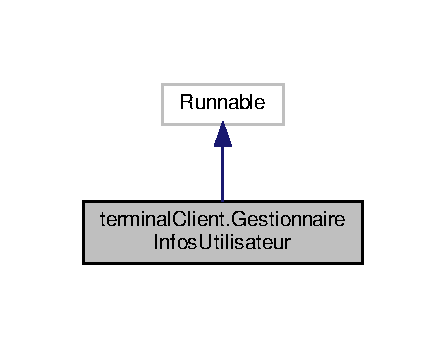
\includegraphics[width=232pt]{classterminalClient_1_1GestionnaireInfosUtilisateur__inherit__graph}
\end{center}
\end{figure}


Collaboration diagram for terminal\+Client.\+Gestionnaire\+Infos\+Utilisateur\+:
\nopagebreak
\begin{figure}[H]
\begin{center}
\leavevmode
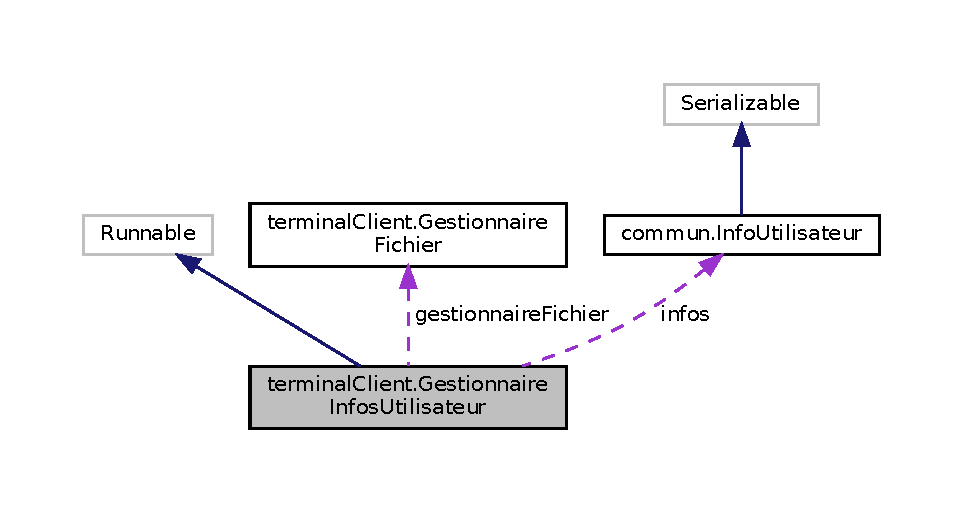
\includegraphics[width=350pt]{classterminalClient_1_1GestionnaireInfosUtilisateur__coll__graph}
\end{center}
\end{figure}
\doxysubsection*{Public Member Functions}
\begin{DoxyCompactItemize}
\item 
\mbox{\hyperlink{classterminalClient_1_1GestionnaireInfosUtilisateur_a8f2c5556445a2c0bcb812234d1026b49}{Gestionnaire\+Infos\+Utilisateur}} (\mbox{\hyperlink{classterminalClient_1_1GestionnaireFichier}{Gestionnaire\+Fichier}} gestionnaire\+Fichier, String ip\+Serveur\+Central, int port\+Serveur\+Central, int port)
\begin{DoxyCompactList}\small\item\em constructeur de la classe. \end{DoxyCompactList}\item 
\mbox{\Hypertarget{classterminalClient_1_1GestionnaireInfosUtilisateur_ad1e9e354a68f58057d1104bd7d4cbdf5}\label{classterminalClient_1_1GestionnaireInfosUtilisateur_ad1e9e354a68f58057d1104bd7d4cbdf5}} 
void \mbox{\hyperlink{classterminalClient_1_1GestionnaireInfosUtilisateur_ad1e9e354a68f58057d1104bd7d4cbdf5}{run}} ()
\begin{DoxyCompactList}\small\item\em méthode pour lancer le Thread. \end{DoxyCompactList}\end{DoxyCompactItemize}


\doxysubsection{Detailed Description}
cette classe va permettre d\textquotesingle{}envoyer régulierement des infos concenrnant l\textquotesingle{}utilisateur au serveur central. 

\doxysubsection{Constructor \& Destructor Documentation}
\mbox{\Hypertarget{classterminalClient_1_1GestionnaireInfosUtilisateur_a8f2c5556445a2c0bcb812234d1026b49}\label{classterminalClient_1_1GestionnaireInfosUtilisateur_a8f2c5556445a2c0bcb812234d1026b49}} 
\index{terminalClient.GestionnaireInfosUtilisateur@{terminalClient.GestionnaireInfosUtilisateur}!GestionnaireInfosUtilisateur@{GestionnaireInfosUtilisateur}}
\index{GestionnaireInfosUtilisateur@{GestionnaireInfosUtilisateur}!terminalClient.GestionnaireInfosUtilisateur@{terminalClient.GestionnaireInfosUtilisateur}}
\doxysubsubsection{\texorpdfstring{GestionnaireInfosUtilisateur()}{GestionnaireInfosUtilisateur()}}
{\footnotesize\ttfamily terminal\+Client.\+Gestionnaire\+Infos\+Utilisateur.\+Gestionnaire\+Infos\+Utilisateur (\begin{DoxyParamCaption}\item[{\mbox{\hyperlink{classterminalClient_1_1GestionnaireFichier}{Gestionnaire\+Fichier}}}]{gestionnaire\+Fichier,  }\item[{String}]{ip\+Serveur\+Central,  }\item[{int}]{port\+Serveur\+Central,  }\item[{int}]{port }\end{DoxyParamCaption})\hspace{0.3cm}{\ttfamily [inline]}}



constructeur de la classe. 


\begin{DoxyParams}{Parameters}
{\em gestionnaire\+Fichier} & le gestionnaire de fichier. \\
\hline
{\em ip\+Serveur\+Central} & l\textquotesingle{}ip du serveur central. \\
\hline
{\em port\+Serveur\+Central} & le port du serveur central. \\
\hline
{\em port} & d\textquotesingle{}écoute de la fonctionnalité serveur du client. \\
\hline
\end{DoxyParams}


The documentation for this class was generated from the following file\+:\begin{DoxyCompactItemize}
\item 
Gestionnaire\+Infos\+Utilisateur.\+java\end{DoxyCompactItemize}

\hypertarget{classgestionnaireRequete_1_1GestionnaireRequetes}{}\doxysection{gestionnaire\+Requete.\+Gestionnaire\+Requetes Class Reference}
\label{classgestionnaireRequete_1_1GestionnaireRequetes}\index{gestionnaireRequete.GestionnaireRequetes@{gestionnaireRequete.GestionnaireRequetes}}


Cette classe abstrait permet de gérer les requêtes d\textquotesingle{}un client.  




Inheritance diagram for gestionnaire\+Requete.\+Gestionnaire\+Requetes\+:
\nopagebreak
\begin{figure}[H]
\begin{center}
\leavevmode
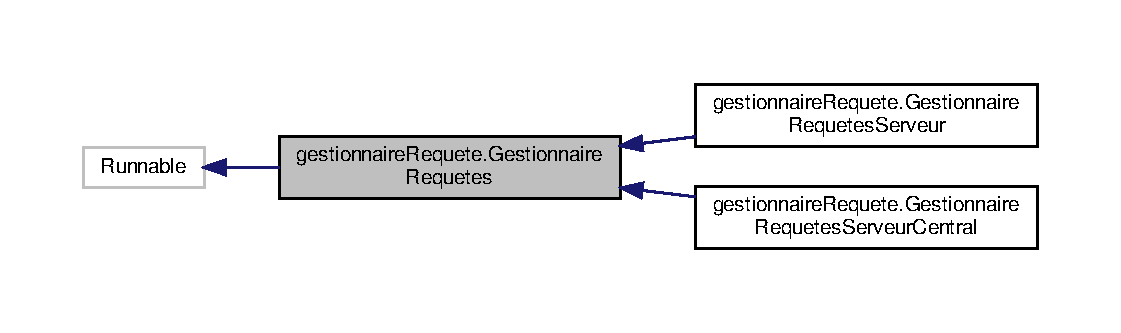
\includegraphics[width=350pt]{classgestionnaireRequete_1_1GestionnaireRequetes__inherit__graph}
\end{center}
\end{figure}


Collaboration diagram for gestionnaire\+Requete.\+Gestionnaire\+Requetes\+:
\nopagebreak
\begin{figure}[H]
\begin{center}
\leavevmode
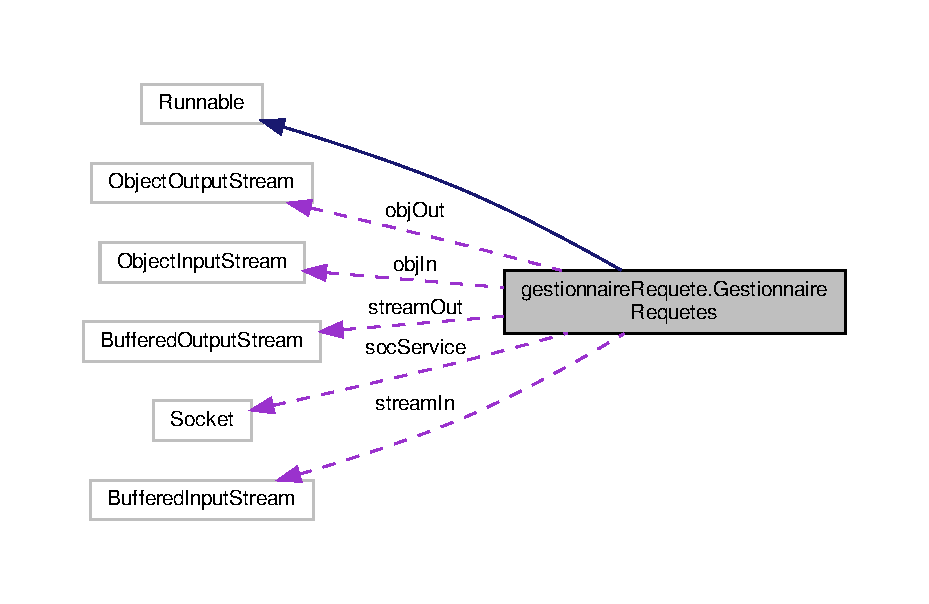
\includegraphics[width=350pt]{classgestionnaireRequete_1_1GestionnaireRequetes__coll__graph}
\end{center}
\end{figure}
\doxysubsection*{Public Member Functions}
\begin{DoxyCompactItemize}
\item 
\mbox{\hyperlink{classgestionnaireRequete_1_1GestionnaireRequetes_a30364d904d0ab798250e1f7a0a7e9465}{Gestionnaire\+Requetes}} (Socket soc\+Service)  throws I\+O\+Exception 
\begin{DoxyCompactList}\small\item\em constructeur de \mbox{\hyperlink{classgestionnaireRequete_1_1GestionnaireRequetes}{Gestionnaire\+Requetes}}. \end{DoxyCompactList}\item 
\mbox{\Hypertarget{classgestionnaireRequete_1_1GestionnaireRequetes_a2bdb6af7bf6fc711b4565890899b8b6d}\label{classgestionnaireRequete_1_1GestionnaireRequetes_a2bdb6af7bf6fc711b4565890899b8b6d}} 
void \mbox{\hyperlink{classgestionnaireRequete_1_1GestionnaireRequetes_a2bdb6af7bf6fc711b4565890899b8b6d}{run}} ()
\begin{DoxyCompactList}\small\item\em methode pour lancer le Thread. \end{DoxyCompactList}\end{DoxyCompactItemize}
\doxysubsection*{Protected Member Functions}
\begin{DoxyCompactItemize}
\item 
abstract void \mbox{\hyperlink{classgestionnaireRequete_1_1GestionnaireRequetes_a703068945b171f22015fb5cc1f880190}{servir\+Client}} (String requete)  throws I\+O\+Exception
\begin{DoxyCompactList}\small\item\em cette fonction abstraite répond aux demande du client. \end{DoxyCompactList}\item 
String \mbox{\hyperlink{classgestionnaireRequete_1_1GestionnaireRequetes_a71eceb6b3b7236615f117e0ddf75896c}{lire\+Requete\+Client}} ()  throws I\+O\+Exception 
\begin{DoxyCompactList}\small\item\em Cette méthode va lire une requête envoyée par le client. \end{DoxyCompactList}\end{DoxyCompactItemize}
\doxysubsection*{Protected Attributes}
\begin{DoxyCompactItemize}
\item 
\mbox{\Hypertarget{classgestionnaireRequete_1_1GestionnaireRequetes_a52fc455531cd68bc9495d0ad0351f6d9}\label{classgestionnaireRequete_1_1GestionnaireRequetes_a52fc455531cd68bc9495d0ad0351f6d9}} 
Socket {\bfseries soc\+Service}
\item 
\mbox{\Hypertarget{classgestionnaireRequete_1_1GestionnaireRequetes_ac0c4788d552f54cca0bf4d73e9c57300}\label{classgestionnaireRequete_1_1GestionnaireRequetes_ac0c4788d552f54cca0bf4d73e9c57300}} 
Buffered\+Input\+Stream {\bfseries stream\+In}
\item 
\mbox{\Hypertarget{classgestionnaireRequete_1_1GestionnaireRequetes_a616ecc1b5abfa7363497f84d2e17342a}\label{classgestionnaireRequete_1_1GestionnaireRequetes_a616ecc1b5abfa7363497f84d2e17342a}} 
Buffered\+Output\+Stream {\bfseries stream\+Out}
\item 
\mbox{\Hypertarget{classgestionnaireRequete_1_1GestionnaireRequetes_a505d88bbe17a513d54c8e30b878df7f9}\label{classgestionnaireRequete_1_1GestionnaireRequetes_a505d88bbe17a513d54c8e30b878df7f9}} 
Object\+Input\+Stream {\bfseries obj\+In}
\item 
\mbox{\Hypertarget{classgestionnaireRequete_1_1GestionnaireRequetes_a775bd6fdb30b8c0c2405c6e6b7800bd6}\label{classgestionnaireRequete_1_1GestionnaireRequetes_a775bd6fdb30b8c0c2405c6e6b7800bd6}} 
Object\+Output\+Stream {\bfseries obj\+Out}
\item 
\mbox{\Hypertarget{classgestionnaireRequete_1_1GestionnaireRequetes_a557720ba61fd14d2a12f81743fc1febe}\label{classgestionnaireRequete_1_1GestionnaireRequetes_a557720ba61fd14d2a12f81743fc1febe}} 
String {\bfseries requete}
\end{DoxyCompactItemize}


\doxysubsection{Detailed Description}
Cette classe abstrait permet de gérer les requêtes d\textquotesingle{}un client. 

\doxysubsection{Constructor \& Destructor Documentation}
\mbox{\Hypertarget{classgestionnaireRequete_1_1GestionnaireRequetes_a30364d904d0ab798250e1f7a0a7e9465}\label{classgestionnaireRequete_1_1GestionnaireRequetes_a30364d904d0ab798250e1f7a0a7e9465}} 
\index{gestionnaireRequete.GestionnaireRequetes@{gestionnaireRequete.GestionnaireRequetes}!GestionnaireRequetes@{GestionnaireRequetes}}
\index{GestionnaireRequetes@{GestionnaireRequetes}!gestionnaireRequete.GestionnaireRequetes@{gestionnaireRequete.GestionnaireRequetes}}
\doxysubsubsection{\texorpdfstring{GestionnaireRequetes()}{GestionnaireRequetes()}}
{\footnotesize\ttfamily gestionnaire\+Requete.\+Gestionnaire\+Requetes.\+Gestionnaire\+Requetes (\begin{DoxyParamCaption}\item[{Socket}]{soc\+Service }\end{DoxyParamCaption}) throws I\+O\+Exception\hspace{0.3cm}{\ttfamily [inline]}}



constructeur de \mbox{\hyperlink{classgestionnaireRequete_1_1GestionnaireRequetes}{Gestionnaire\+Requetes}}. 


\begin{DoxyParams}{Parameters}
{\em soc\+Service} & la socket de service qui permet de communiquer avec le client. \\
\hline
\end{DoxyParams}

\begin{DoxyExceptions}{Exceptions}
{\em I\+O\+Exception} & exception qui survient à la création du stream \\
\hline
\end{DoxyExceptions}


\doxysubsection{Member Function Documentation}
\mbox{\Hypertarget{classgestionnaireRequete_1_1GestionnaireRequetes_a71eceb6b3b7236615f117e0ddf75896c}\label{classgestionnaireRequete_1_1GestionnaireRequetes_a71eceb6b3b7236615f117e0ddf75896c}} 
\index{gestionnaireRequete.GestionnaireRequetes@{gestionnaireRequete.GestionnaireRequetes}!lireRequeteClient@{lireRequeteClient}}
\index{lireRequeteClient@{lireRequeteClient}!gestionnaireRequete.GestionnaireRequetes@{gestionnaireRequete.GestionnaireRequetes}}
\doxysubsubsection{\texorpdfstring{lireRequeteClient()}{lireRequeteClient()}}
{\footnotesize\ttfamily String gestionnaire\+Requete.\+Gestionnaire\+Requetes.\+lire\+Requete\+Client (\begin{DoxyParamCaption}{ }\end{DoxyParamCaption}) throws I\+O\+Exception\hspace{0.3cm}{\ttfamily [inline]}, {\ttfamily [protected]}}



Cette méthode va lire une requête envoyée par le client. 

\begin{DoxyReturn}{Returns}
retourne la requête sous forme de chaine de caractères. 
\end{DoxyReturn}

\begin{DoxyExceptions}{Exceptions}
{\em I\+O\+Exception} & léve une exception si la fonction n\textquotesingle{}arrive pas à lire la requête envoyé par le client. \\
\hline
\end{DoxyExceptions}
\mbox{\Hypertarget{classgestionnaireRequete_1_1GestionnaireRequetes_a703068945b171f22015fb5cc1f880190}\label{classgestionnaireRequete_1_1GestionnaireRequetes_a703068945b171f22015fb5cc1f880190}} 
\index{gestionnaireRequete.GestionnaireRequetes@{gestionnaireRequete.GestionnaireRequetes}!servirClient@{servirClient}}
\index{servirClient@{servirClient}!gestionnaireRequete.GestionnaireRequetes@{gestionnaireRequete.GestionnaireRequetes}}
\doxysubsubsection{\texorpdfstring{servirClient()}{servirClient()}}
{\footnotesize\ttfamily abstract void gestionnaire\+Requete.\+Gestionnaire\+Requetes.\+servir\+Client (\begin{DoxyParamCaption}\item[{String}]{requete }\end{DoxyParamCaption}) throws I\+O\+Exception\hspace{0.3cm}{\ttfamily [abstract]}, {\ttfamily [protected]}}



cette fonction abstraite répond aux demande du client. 


\begin{DoxyParams}{Parameters}
{\em requete} & requete demandé par l\textquotesingle{}utilisateur \\
\hline
\end{DoxyParams}

\begin{DoxyExceptions}{Exceptions}
{\em I\+O\+Exception} & exceptions qui peuvent être remontées en cas de problème. \\
\hline
\end{DoxyExceptions}


Reimplemented in \mbox{\hyperlink{classgestionnaireRequete_1_1GestionnaireRequetesServeurCentral_a7e4ac9416e0d8c5d68857775aea589d6}{gestionnaire\+Requete.\+Gestionnaire\+Requetes\+Serveur\+Central}}, and \mbox{\hyperlink{classgestionnaireRequete_1_1GestionnaireRequetesServeur_a20c9f53be4a6126872c97d813afb1b51}{gestionnaire\+Requete.\+Gestionnaire\+Requetes\+Serveur}}.



The documentation for this class was generated from the following file\+:\begin{DoxyCompactItemize}
\item 
Gestionnaire\+Requetes.\+java\end{DoxyCompactItemize}

\hypertarget{classgestionnaireRequete_1_1GestionnaireRequetesServeur}{}\doxysection{gestionnaire\+Requete.\+Gestionnaire\+Requetes\+Serveur Class Reference}
\label{classgestionnaireRequete_1_1GestionnaireRequetesServeur}\index{gestionnaireRequete.GestionnaireRequetesServeur@{gestionnaireRequete.GestionnaireRequetesServeur}}


Cette classe gere les requêtes d\textquotesingle{}un client pour la fonctionnalité \char`\"{}\+Serveur\char`\"{} de chaque client.  




Inheritance diagram for gestionnaire\+Requete.\+Gestionnaire\+Requetes\+Serveur\+:
\nopagebreak
\begin{figure}[H]
\begin{center}
\leavevmode
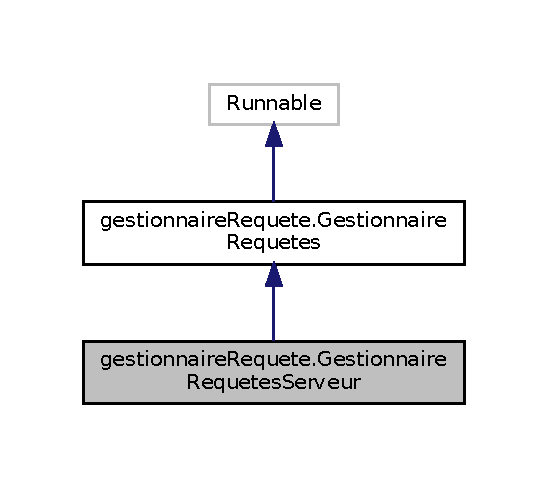
\includegraphics[width=263pt]{classgestionnaireRequete_1_1GestionnaireRequetesServeur__inherit__graph}
\end{center}
\end{figure}


Collaboration diagram for gestionnaire\+Requete.\+Gestionnaire\+Requetes\+Serveur\+:
\nopagebreak
\begin{figure}[H]
\begin{center}
\leavevmode
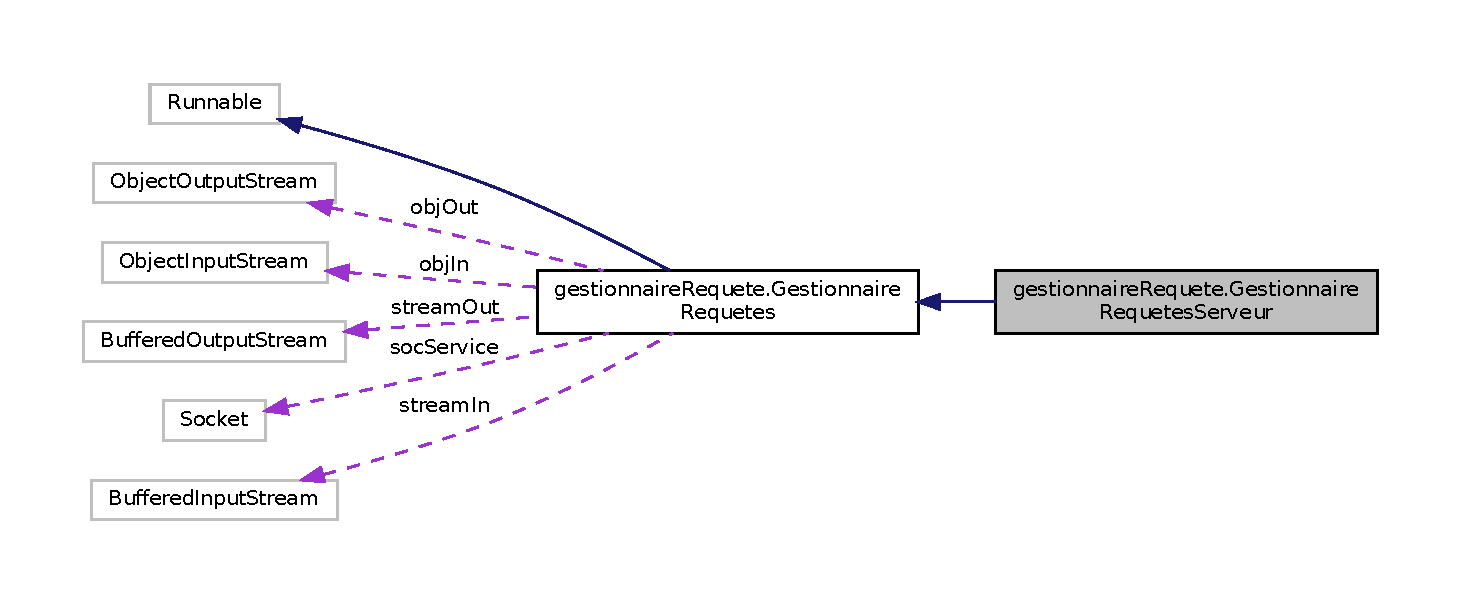
\includegraphics[width=350pt]{classgestionnaireRequete_1_1GestionnaireRequetesServeur__coll__graph}
\end{center}
\end{figure}
\doxysubsection*{Public Member Functions}
\begin{DoxyCompactItemize}
\item 
\mbox{\hyperlink{classgestionnaireRequete_1_1GestionnaireRequetesServeur_a80cb3c0cc910d1678916bd93ea4175d3}{Gestionnaire\+Requetes\+Serveur}} (Socket soc\+Service, \mbox{\hyperlink{classterminalClient_1_1GestionnaireFichier}{Gestionnaire\+Fichier}} gestionnaire\+Fichier)  throws I\+O\+Exception 
\begin{DoxyCompactList}\small\item\em constructeur de \mbox{\hyperlink{classgestionnaireRequete_1_1GestionnaireRequetesServeur}{Gestionnaire\+Requetes\+Serveur}}. \end{DoxyCompactList}\end{DoxyCompactItemize}
\doxysubsection*{Protected Member Functions}
\begin{DoxyCompactItemize}
\item 
void \mbox{\hyperlink{classgestionnaireRequete_1_1GestionnaireRequetesServeur_a20c9f53be4a6126872c97d813afb1b51}{servir\+Client}} (String requete)  throws I\+O\+Exception 
\begin{DoxyCompactList}\small\item\em cette fonction répond aux demande du client. \end{DoxyCompactList}\end{DoxyCompactItemize}
\doxysubsection*{Additional Inherited Members}


\doxysubsection{Detailed Description}
Cette classe gere les requêtes d\textquotesingle{}un client pour la fonctionnalité \char`\"{}\+Serveur\char`\"{} de chaque client. 

\doxysubsection{Constructor \& Destructor Documentation}
\mbox{\Hypertarget{classgestionnaireRequete_1_1GestionnaireRequetesServeur_a80cb3c0cc910d1678916bd93ea4175d3}\label{classgestionnaireRequete_1_1GestionnaireRequetesServeur_a80cb3c0cc910d1678916bd93ea4175d3}} 
\index{gestionnaireRequete.GestionnaireRequetesServeur@{gestionnaireRequete.GestionnaireRequetesServeur}!GestionnaireRequetesServeur@{GestionnaireRequetesServeur}}
\index{GestionnaireRequetesServeur@{GestionnaireRequetesServeur}!gestionnaireRequete.GestionnaireRequetesServeur@{gestionnaireRequete.GestionnaireRequetesServeur}}
\doxysubsubsection{\texorpdfstring{GestionnaireRequetesServeur()}{GestionnaireRequetesServeur()}}
{\footnotesize\ttfamily gestionnaire\+Requete.\+Gestionnaire\+Requetes\+Serveur.\+Gestionnaire\+Requetes\+Serveur (\begin{DoxyParamCaption}\item[{Socket}]{soc\+Service,  }\item[{\mbox{\hyperlink{classterminalClient_1_1GestionnaireFichier}{Gestionnaire\+Fichier}}}]{gestionnaire\+Fichier }\end{DoxyParamCaption}) throws I\+O\+Exception\hspace{0.3cm}{\ttfamily [inline]}}



constructeur de \mbox{\hyperlink{classgestionnaireRequete_1_1GestionnaireRequetesServeur}{Gestionnaire\+Requetes\+Serveur}}. 


\begin{DoxyParams}{Parameters}
{\em soc\+Service} & la socket de service qui permet de communiquer avec le client. \\
\hline
\end{DoxyParams}

\begin{DoxyExceptions}{Exceptions}
{\em I\+O\+Exception} & exception qui survient à la création du stream \\
\hline
\end{DoxyExceptions}


\doxysubsection{Member Function Documentation}
\mbox{\Hypertarget{classgestionnaireRequete_1_1GestionnaireRequetesServeur_a20c9f53be4a6126872c97d813afb1b51}\label{classgestionnaireRequete_1_1GestionnaireRequetesServeur_a20c9f53be4a6126872c97d813afb1b51}} 
\index{gestionnaireRequete.GestionnaireRequetesServeur@{gestionnaireRequete.GestionnaireRequetesServeur}!servirClient@{servirClient}}
\index{servirClient@{servirClient}!gestionnaireRequete.GestionnaireRequetesServeur@{gestionnaireRequete.GestionnaireRequetesServeur}}
\doxysubsubsection{\texorpdfstring{servirClient()}{servirClient()}}
{\footnotesize\ttfamily void gestionnaire\+Requete.\+Gestionnaire\+Requetes\+Serveur.\+servir\+Client (\begin{DoxyParamCaption}\item[{String}]{requete }\end{DoxyParamCaption}) throws I\+O\+Exception\hspace{0.3cm}{\ttfamily [inline]}, {\ttfamily [protected]}}



cette fonction répond aux demande du client. 


\begin{DoxyParams}{Parameters}
{\em requete} & requete demandé par l\textquotesingle{}utilisateur \\
\hline
\end{DoxyParams}

\begin{DoxyExceptions}{Exceptions}
{\em I\+O\+Exception} & exception levée par la méthode envoyer\+Liste() \\
\hline
\end{DoxyExceptions}


Reimplemented from \mbox{\hyperlink{classgestionnaireRequete_1_1GestionnaireRequetes_a703068945b171f22015fb5cc1f880190}{gestionnaire\+Requete.\+Gestionnaire\+Requetes}}.



The documentation for this class was generated from the following file\+:\begin{DoxyCompactItemize}
\item 
Gestionnaire\+Requetes\+Serveur.\+java\end{DoxyCompactItemize}

\hypertarget{classgestionnaireRequete_1_1GestionnaireRequetesServeurCentral}{}\section{gestionnaire\+Requete.\+Gestionnaire\+Requetes\+Serveur\+Central Class Reference}
\label{classgestionnaireRequete_1_1GestionnaireRequetesServeurCentral}\index{gestionnaire\+Requete.\+Gestionnaire\+Requetes\+Serveur\+Central@{gestionnaire\+Requete.\+Gestionnaire\+Requetes\+Serveur\+Central}}


Cette classe gere les requêtes d\textquotesingle{}un client vers le serveur central.  




Inheritance diagram for gestionnaire\+Requete.\+Gestionnaire\+Requetes\+Serveur\+Central\+:\nopagebreak
\begin{figure}[H]
\begin{center}
\leavevmode
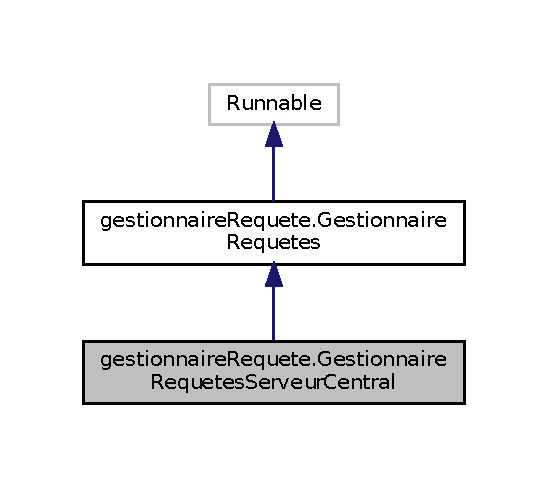
\includegraphics[width=244pt]{classgestionnaireRequete_1_1GestionnaireRequetesServeurCentral__inherit__graph}
\end{center}
\end{figure}


Collaboration diagram for gestionnaire\+Requete.\+Gestionnaire\+Requetes\+Serveur\+Central\+:\nopagebreak
\begin{figure}[H]
\begin{center}
\leavevmode
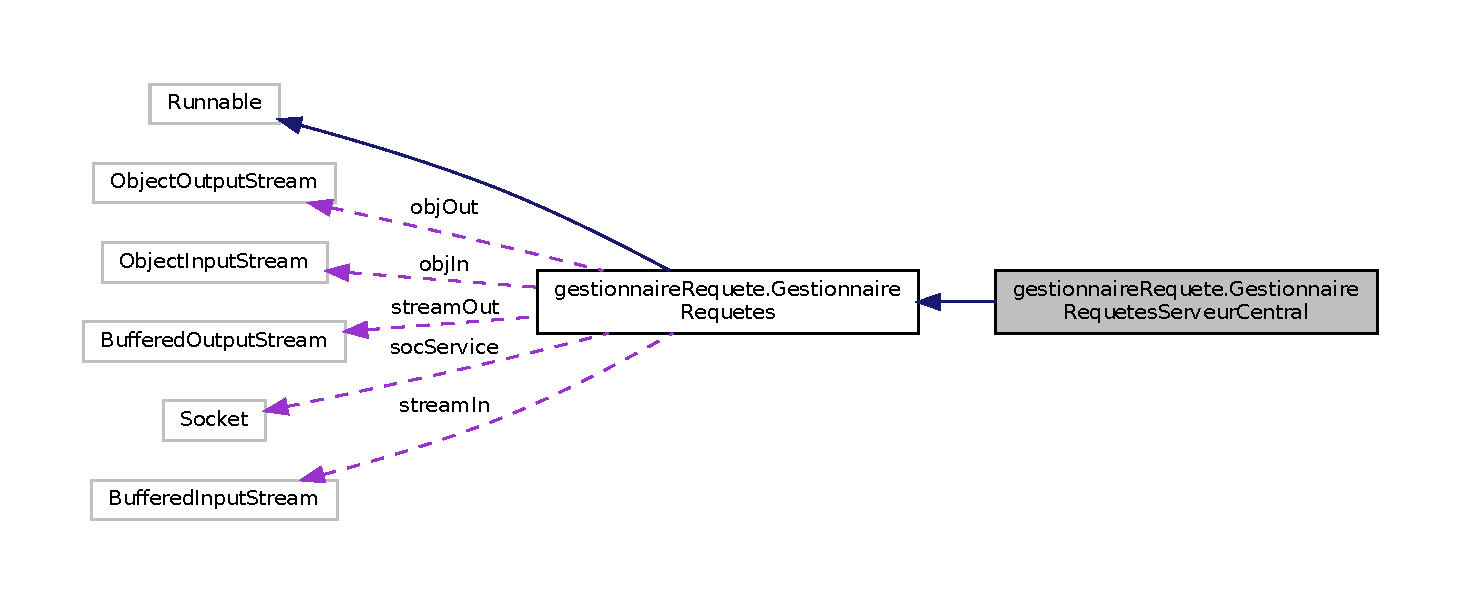
\includegraphics[width=350pt]{classgestionnaireRequete_1_1GestionnaireRequetesServeurCentral__coll__graph}
\end{center}
\end{figure}
\subsection*{Public Member Functions}
\begin{DoxyCompactItemize}
\item 
\hyperlink{classgestionnaireRequete_1_1GestionnaireRequetesServeurCentral_a51ac22ccddf0c79c588f596118dd39ae}{Gestionnaire\+Requetes\+Serveur\+Central} (Socket soc\+Service)  throws I\+O\+Exception 
\begin{DoxyCompactList}\small\item\em constructeur de \hyperlink{classgestionnaireRequete_1_1GestionnaireRequetesServeur}{Gestionnaire\+Requetes\+Serveur}. \end{DoxyCompactList}\end{DoxyCompactItemize}
\subsection*{Protected Member Functions}
\begin{DoxyCompactItemize}
\item 
void \hyperlink{classgestionnaireRequete_1_1GestionnaireRequetesServeurCentral_a7e4ac9416e0d8c5d68857775aea589d6}{servir\+Client} (String requete)  throws I\+O\+Exception 
\begin{DoxyCompactList}\small\item\em cette fonction répond aux demande du client. \end{DoxyCompactList}\end{DoxyCompactItemize}
\subsection*{Additional Inherited Members}


\subsection{Detailed Description}
Cette classe gere les requêtes d\textquotesingle{}un client vers le serveur central. 

\subsection{Constructor \& Destructor Documentation}
\mbox{\Hypertarget{classgestionnaireRequete_1_1GestionnaireRequetesServeurCentral_a51ac22ccddf0c79c588f596118dd39ae}\label{classgestionnaireRequete_1_1GestionnaireRequetesServeurCentral_a51ac22ccddf0c79c588f596118dd39ae}} 
\index{gestionnaire\+Requete\+::\+Gestionnaire\+Requetes\+Serveur\+Central@{gestionnaire\+Requete\+::\+Gestionnaire\+Requetes\+Serveur\+Central}!Gestionnaire\+Requetes\+Serveur\+Central@{Gestionnaire\+Requetes\+Serveur\+Central}}
\index{Gestionnaire\+Requetes\+Serveur\+Central@{Gestionnaire\+Requetes\+Serveur\+Central}!gestionnaire\+Requete\+::\+Gestionnaire\+Requetes\+Serveur\+Central@{gestionnaire\+Requete\+::\+Gestionnaire\+Requetes\+Serveur\+Central}}
\subsubsection{\texorpdfstring{Gestionnaire\+Requetes\+Serveur\+Central()}{GestionnaireRequetesServeurCentral()}}
{\footnotesize\ttfamily gestionnaire\+Requete.\+Gestionnaire\+Requetes\+Serveur\+Central.\+Gestionnaire\+Requetes\+Serveur\+Central (\begin{DoxyParamCaption}\item[{Socket}]{soc\+Service }\end{DoxyParamCaption}) throws I\+O\+Exception\hspace{0.3cm}{\ttfamily [inline]}}



constructeur de \hyperlink{classgestionnaireRequete_1_1GestionnaireRequetesServeur}{Gestionnaire\+Requetes\+Serveur}. 


\begin{DoxyParams}{Parameters}
{\em soc\+Service} & la socket de service qui permet de communiquer avec le client. \\
\hline
\end{DoxyParams}

\begin{DoxyExceptions}{Exceptions}
{\em I\+O\+Exception} & exception qui survient à la création du stream \\
\hline
\end{DoxyExceptions}


\subsection{Member Function Documentation}
\mbox{\Hypertarget{classgestionnaireRequete_1_1GestionnaireRequetesServeurCentral_a7e4ac9416e0d8c5d68857775aea589d6}\label{classgestionnaireRequete_1_1GestionnaireRequetesServeurCentral_a7e4ac9416e0d8c5d68857775aea589d6}} 
\index{gestionnaire\+Requete\+::\+Gestionnaire\+Requetes\+Serveur\+Central@{gestionnaire\+Requete\+::\+Gestionnaire\+Requetes\+Serveur\+Central}!servir\+Client@{servir\+Client}}
\index{servir\+Client@{servir\+Client}!gestionnaire\+Requete\+::\+Gestionnaire\+Requetes\+Serveur\+Central@{gestionnaire\+Requete\+::\+Gestionnaire\+Requetes\+Serveur\+Central}}
\subsubsection{\texorpdfstring{servir\+Client()}{servirClient()}}
{\footnotesize\ttfamily void gestionnaire\+Requete.\+Gestionnaire\+Requetes\+Serveur\+Central.\+servir\+Client (\begin{DoxyParamCaption}\item[{String}]{requete }\end{DoxyParamCaption}) throws I\+O\+Exception\hspace{0.3cm}{\ttfamily [inline]}, {\ttfamily [protected]}}



cette fonction répond aux demande du client. 


\begin{DoxyParams}{Parameters}
{\em requete} & requete demandé par l\textquotesingle{}utilisateur \\
\hline
\end{DoxyParams}

\begin{DoxyExceptions}{Exceptions}
{\em I\+O\+Exception} & exception levée par la méthode envoyer\+Liste() \\
\hline
\end{DoxyExceptions}


The documentation for this class was generated from the following file\+:\begin{DoxyCompactItemize}
\item 
Gestionnaire\+Requetes\+Serveur\+Central.\+java\end{DoxyCompactItemize}

\hypertarget{classcommun_1_1InfoUtilisateur}{}\doxysection{commun.\+Info\+Utilisateur Class Reference}
\label{classcommun_1_1InfoUtilisateur}\index{commun.InfoUtilisateur@{commun.InfoUtilisateur}}


cette classe permet de stocker les informations sur un utilisateur (ip, port, liste des fichiers qu\textquotesingle{}il possède et quel parties de ces fichiers il possède)  




Inheritance diagram for commun.\+Info\+Utilisateur\+:
\nopagebreak
\begin{figure}[H]
\begin{center}
\leavevmode
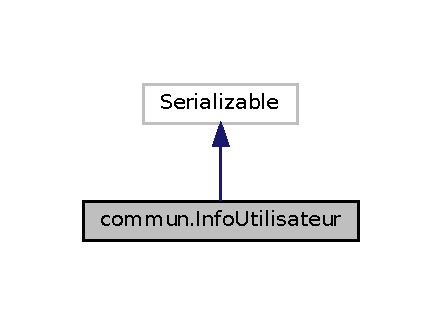
\includegraphics[width=212pt]{classcommun_1_1InfoUtilisateur__inherit__graph}
\end{center}
\end{figure}


Collaboration diagram for commun.\+Info\+Utilisateur\+:
\nopagebreak
\begin{figure}[H]
\begin{center}
\leavevmode
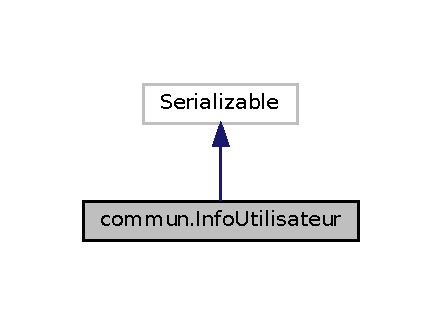
\includegraphics[width=212pt]{classcommun_1_1InfoUtilisateur__coll__graph}
\end{center}
\end{figure}
\doxysubsection*{Public Member Functions}
\begin{DoxyCompactItemize}
\item 
\mbox{\hyperlink{classcommun_1_1InfoUtilisateur_aaa6fb8bb0211678aad4fe5343d36485e}{Info\+Utilisateur}} (String ip, int port)
\begin{DoxyCompactList}\small\item\em constructeur de la classe. \end{DoxyCompactList}\item 
String \mbox{\hyperlink{classcommun_1_1InfoUtilisateur_acdf31d84ce570faa468b6bae8416e998}{get\+Ip}} ()
\begin{DoxyCompactList}\small\item\em permet d\textquotesingle{}obtenir l\textquotesingle{}ip de l\textquotesingle{}utilisateur. \end{DoxyCompactList}\item 
int \mbox{\hyperlink{classcommun_1_1InfoUtilisateur_a534d959e66e5495fb67f4289573d7be9}{get\+Port}} ()
\begin{DoxyCompactList}\small\item\em permet d\textquotesingle{}obtenir le port d\textquotesingle{}écoute de l\textquotesingle{}utilisateur. \end{DoxyCompactList}\item 
Hash\+Map$<$ String, Long $>$ \mbox{\hyperlink{classcommun_1_1InfoUtilisateur_a792f0a8d202c280ca41da46151265dea}{obtenir\+La\+Liste\+Des\+Fichiers\+Complets}} ()
\begin{DoxyCompactList}\small\item\em permet de récuperer la liste des fichiers complets de l\textquotesingle{}utilisateur. \end{DoxyCompactList}\item 
void \mbox{\hyperlink{classcommun_1_1InfoUtilisateur_a49464d9eecf82d8768449eabc848aa39}{ajouter\+Fichier}} (String nom\+Fichier, \mbox{\hyperlink{classcommun_1_1ListeDeBlocs}{Liste\+De\+Blocs}} liste\+De\+Blocs)
\begin{DoxyCompactList}\small\item\em ajoute un fichier et la liste des blocs de ce fichier que l\textquotesingle{}utilisateur possede. \end{DoxyCompactList}\item 
boolean \mbox{\hyperlink{classcommun_1_1InfoUtilisateur_ab120b90f5b5cf07fc6ebc9b34488e3b3}{detient\+Le\+Fichier}} (String nom\+Fichier)
\begin{DoxyCompactList}\small\item\em permet de savoir si l\textquotesingle{}utilisateur detient un fichier spécifique. \end{DoxyCompactList}\item 
\mbox{\hyperlink{classcommun_1_1ListeDeBlocs}{Liste\+De\+Blocs}} \mbox{\hyperlink{classcommun_1_1InfoUtilisateur_a9f1e697ade23c76e070c55e03492b085}{bloc\+Du\+Fichier}} (String nom\+Fichier)
\begin{DoxyCompactList}\small\item\em permet d\textquotesingle{}obtenir la liste de bloc d\textquotesingle{}un fichier que l\textquotesingle{}utilisateur posséde. \end{DoxyCompactList}\item 
\mbox{\Hypertarget{classcommun_1_1InfoUtilisateur_af24c4b39eb5d42019c658e37819a2395}\label{classcommun_1_1InfoUtilisateur_af24c4b39eb5d42019c658e37819a2395}} 
String \mbox{\hyperlink{classcommun_1_1InfoUtilisateur_af24c4b39eb5d42019c658e37819a2395}{to\+String}} ()
\begin{DoxyCompactList}\small\item\em methode pour obtenir une description de l\textquotesingle{}objet l\textquotesingle{}info utilisateur principalement utilisé pour debuger et pour afficher des informations. \end{DoxyCompactList}\end{DoxyCompactItemize}


\doxysubsection{Detailed Description}
cette classe permet de stocker les informations sur un utilisateur (ip, port, liste des fichiers qu\textquotesingle{}il possède et quel parties de ces fichiers il possède) 

\doxysubsection{Constructor \& Destructor Documentation}
\mbox{\Hypertarget{classcommun_1_1InfoUtilisateur_aaa6fb8bb0211678aad4fe5343d36485e}\label{classcommun_1_1InfoUtilisateur_aaa6fb8bb0211678aad4fe5343d36485e}} 
\index{commun.InfoUtilisateur@{commun.InfoUtilisateur}!InfoUtilisateur@{InfoUtilisateur}}
\index{InfoUtilisateur@{InfoUtilisateur}!commun.InfoUtilisateur@{commun.InfoUtilisateur}}
\doxysubsubsection{\texorpdfstring{InfoUtilisateur()}{InfoUtilisateur()}}
{\footnotesize\ttfamily commun.\+Info\+Utilisateur.\+Info\+Utilisateur (\begin{DoxyParamCaption}\item[{String}]{ip,  }\item[{int}]{port }\end{DoxyParamCaption})\hspace{0.3cm}{\ttfamily [inline]}}



constructeur de la classe. 


\begin{DoxyParams}{Parameters}
{\em ip} & ip de l\textquotesingle{}utilisateur \\
\hline
{\em port} & port d\textquotesingle{}écoute de l\textquotesingle{}utilisateur. \\
\hline
\end{DoxyParams}


\doxysubsection{Member Function Documentation}
\mbox{\Hypertarget{classcommun_1_1InfoUtilisateur_a49464d9eecf82d8768449eabc848aa39}\label{classcommun_1_1InfoUtilisateur_a49464d9eecf82d8768449eabc848aa39}} 
\index{commun.InfoUtilisateur@{commun.InfoUtilisateur}!ajouterFichier@{ajouterFichier}}
\index{ajouterFichier@{ajouterFichier}!commun.InfoUtilisateur@{commun.InfoUtilisateur}}
\doxysubsubsection{\texorpdfstring{ajouterFichier()}{ajouterFichier()}}
{\footnotesize\ttfamily void commun.\+Info\+Utilisateur.\+ajouter\+Fichier (\begin{DoxyParamCaption}\item[{String}]{nom\+Fichier,  }\item[{\mbox{\hyperlink{classcommun_1_1ListeDeBlocs}{Liste\+De\+Blocs}}}]{liste\+De\+Blocs }\end{DoxyParamCaption})\hspace{0.3cm}{\ttfamily [inline]}}



ajoute un fichier et la liste des blocs de ce fichier que l\textquotesingle{}utilisateur possede. 


\begin{DoxyParams}{Parameters}
{\em nom\+Fichier} & le nom du fichier. \\
\hline
{\em liste\+De\+Blocs} & la liste des blocs du fichier. \\
\hline
\end{DoxyParams}
\mbox{\Hypertarget{classcommun_1_1InfoUtilisateur_a9f1e697ade23c76e070c55e03492b085}\label{classcommun_1_1InfoUtilisateur_a9f1e697ade23c76e070c55e03492b085}} 
\index{commun.InfoUtilisateur@{commun.InfoUtilisateur}!blocDuFichier@{blocDuFichier}}
\index{blocDuFichier@{blocDuFichier}!commun.InfoUtilisateur@{commun.InfoUtilisateur}}
\doxysubsubsection{\texorpdfstring{blocDuFichier()}{blocDuFichier()}}
{\footnotesize\ttfamily \mbox{\hyperlink{classcommun_1_1ListeDeBlocs}{Liste\+De\+Blocs}} commun.\+Info\+Utilisateur.\+bloc\+Du\+Fichier (\begin{DoxyParamCaption}\item[{String}]{nom\+Fichier }\end{DoxyParamCaption})\hspace{0.3cm}{\ttfamily [inline]}}



permet d\textquotesingle{}obtenir la liste de bloc d\textquotesingle{}un fichier que l\textquotesingle{}utilisateur posséde. 


\begin{DoxyParams}{Parameters}
{\em nom\+Fichier} & le nom du fichier dont on souhaite obtenir la liste de blocs. \\
\hline
\end{DoxyParams}
\begin{DoxyReturn}{Returns}
renvoie la liste de blocs du fichier de l\textquotesingle{}utilisateur. 
\end{DoxyReturn}
\mbox{\Hypertarget{classcommun_1_1InfoUtilisateur_ab120b90f5b5cf07fc6ebc9b34488e3b3}\label{classcommun_1_1InfoUtilisateur_ab120b90f5b5cf07fc6ebc9b34488e3b3}} 
\index{commun.InfoUtilisateur@{commun.InfoUtilisateur}!detientLeFichier@{detientLeFichier}}
\index{detientLeFichier@{detientLeFichier}!commun.InfoUtilisateur@{commun.InfoUtilisateur}}
\doxysubsubsection{\texorpdfstring{detientLeFichier()}{detientLeFichier()}}
{\footnotesize\ttfamily boolean commun.\+Info\+Utilisateur.\+detient\+Le\+Fichier (\begin{DoxyParamCaption}\item[{String}]{nom\+Fichier }\end{DoxyParamCaption})\hspace{0.3cm}{\ttfamily [inline]}}



permet de savoir si l\textquotesingle{}utilisateur detient un fichier spécifique. 


\begin{DoxyParams}{Parameters}
{\em nom\+Fichier} & le nom du fichier dont on veut savoir si l\textquotesingle{}utilisateur à une copie. \\
\hline
\end{DoxyParams}
\begin{DoxyReturn}{Returns}
renvoie true si l\textquotesingle{}utilisateur posséde le fichier, sinon renvoie false. 
\end{DoxyReturn}
\mbox{\Hypertarget{classcommun_1_1InfoUtilisateur_acdf31d84ce570faa468b6bae8416e998}\label{classcommun_1_1InfoUtilisateur_acdf31d84ce570faa468b6bae8416e998}} 
\index{commun.InfoUtilisateur@{commun.InfoUtilisateur}!getIp@{getIp}}
\index{getIp@{getIp}!commun.InfoUtilisateur@{commun.InfoUtilisateur}}
\doxysubsubsection{\texorpdfstring{getIp()}{getIp()}}
{\footnotesize\ttfamily String commun.\+Info\+Utilisateur.\+get\+Ip (\begin{DoxyParamCaption}{ }\end{DoxyParamCaption})\hspace{0.3cm}{\ttfamily [inline]}}



permet d\textquotesingle{}obtenir l\textquotesingle{}ip de l\textquotesingle{}utilisateur. 

\begin{DoxyReturn}{Returns}
retourne l\textquotesingle{}ip de l\textquotesingle{}utilisateur. 
\end{DoxyReturn}
\mbox{\Hypertarget{classcommun_1_1InfoUtilisateur_a534d959e66e5495fb67f4289573d7be9}\label{classcommun_1_1InfoUtilisateur_a534d959e66e5495fb67f4289573d7be9}} 
\index{commun.InfoUtilisateur@{commun.InfoUtilisateur}!getPort@{getPort}}
\index{getPort@{getPort}!commun.InfoUtilisateur@{commun.InfoUtilisateur}}
\doxysubsubsection{\texorpdfstring{getPort()}{getPort()}}
{\footnotesize\ttfamily int commun.\+Info\+Utilisateur.\+get\+Port (\begin{DoxyParamCaption}{ }\end{DoxyParamCaption})\hspace{0.3cm}{\ttfamily [inline]}}



permet d\textquotesingle{}obtenir le port d\textquotesingle{}écoute de l\textquotesingle{}utilisateur. 

\begin{DoxyReturn}{Returns}
retourne le port d\textquotesingle{}écoute de l\textquotesingle{}utilisateur. 
\end{DoxyReturn}
\mbox{\Hypertarget{classcommun_1_1InfoUtilisateur_a792f0a8d202c280ca41da46151265dea}\label{classcommun_1_1InfoUtilisateur_a792f0a8d202c280ca41da46151265dea}} 
\index{commun.InfoUtilisateur@{commun.InfoUtilisateur}!obtenirLaListeDesFichiersComplets@{obtenirLaListeDesFichiersComplets}}
\index{obtenirLaListeDesFichiersComplets@{obtenirLaListeDesFichiersComplets}!commun.InfoUtilisateur@{commun.InfoUtilisateur}}
\doxysubsubsection{\texorpdfstring{obtenirLaListeDesFichiersComplets()}{obtenirLaListeDesFichiersComplets()}}
{\footnotesize\ttfamily Hash\+Map$<$String, Long$>$ commun.\+Info\+Utilisateur.\+obtenir\+La\+Liste\+Des\+Fichiers\+Complets (\begin{DoxyParamCaption}{ }\end{DoxyParamCaption})\hspace{0.3cm}{\ttfamily [inline]}}



permet de récuperer la liste des fichiers complets de l\textquotesingle{}utilisateur. 

\begin{DoxyReturn}{Returns}
renvoie la liste des fichiers complets de l\textquotesingle{}utilisateur. 
\end{DoxyReturn}


The documentation for this class was generated from the following file\+:\begin{DoxyCompactItemize}
\item 
Info\+Utilisateur.\+java\end{DoxyCompactItemize}

\hypertarget{classcommun_1_1ListeDeBlocs}{}\doxysection{commun.\+Liste\+De\+Blocs Class Reference}
\label{classcommun_1_1ListeDeBlocs}\index{commun.ListeDeBlocs@{commun.ListeDeBlocs}}


Cette classe représente une liste de bloc d\textquotesingle{}un fichier d\textquotesingle{}un utilisateur.  




Inheritance diagram for commun.\+Liste\+De\+Blocs\+:
\nopagebreak
\begin{figure}[H]
\begin{center}
\leavevmode
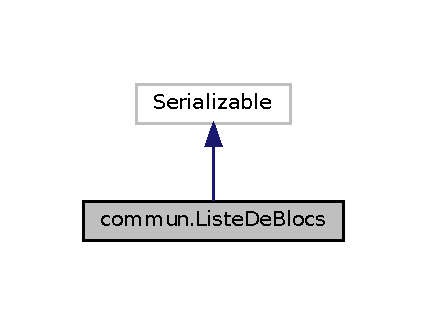
\includegraphics[width=205pt]{classcommun_1_1ListeDeBlocs__inherit__graph}
\end{center}
\end{figure}


Collaboration diagram for commun.\+Liste\+De\+Blocs\+:
\nopagebreak
\begin{figure}[H]
\begin{center}
\leavevmode
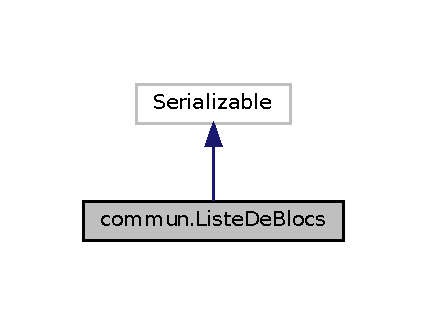
\includegraphics[width=205pt]{classcommun_1_1ListeDeBlocs__coll__graph}
\end{center}
\end{figure}
\doxysubsection*{Public Member Functions}
\begin{DoxyCompactItemize}
\item 
\mbox{\Hypertarget{classcommun_1_1ListeDeBlocs_a558790ed6d6a282260d81f4e7b4789a7}\label{classcommun_1_1ListeDeBlocs_a558790ed6d6a282260d81f4e7b4789a7}} 
\mbox{\hyperlink{classcommun_1_1ListeDeBlocs_a558790ed6d6a282260d81f4e7b4789a7}{Liste\+De\+Blocs}} ()
\begin{DoxyCompactList}\small\item\em constructeur de la classe. \end{DoxyCompactList}\item 
long \mbox{\hyperlink{classcommun_1_1ListeDeBlocs_a52a7e4ed2a3e31d0f1ee2f0c62f8fef0}{obtenir\+Taille\+Du\+Fichier}} ()
\begin{DoxyCompactList}\small\item\em permet d\textquotesingle{}obtenir la taille du fichier \end{DoxyCompactList}\item 
boolean \mbox{\hyperlink{classcommun_1_1ListeDeBlocs_a2a41b1d4ac1c526012a09f415acd5bfe}{detient\+Le\+Bloc}} (int numero\+Du\+Bloc)
\begin{DoxyCompactList}\small\item\em permet de savoir si le fichier à un bloc. \end{DoxyCompactList}\item 
void \mbox{\hyperlink{classcommun_1_1ListeDeBlocs_a31c5d230f4b27f5c94ede5c4104eea1c}{definir\+Taille\+Du\+Fichier}} (long taille\+Du\+Fichier)
\begin{DoxyCompactList}\small\item\em permet de définir la taille du fichier si celui-\/ci est complet. \end{DoxyCompactList}\item 
void \mbox{\hyperlink{classcommun_1_1ListeDeBlocs_a76b292081d24cfdffb66961056e0dab8}{ajouter\+Un\+Bloc}} (int numero)
\begin{DoxyCompactList}\small\item\em ajouter un nouveau bloc à la liste des blocs. \end{DoxyCompactList}\item 
\mbox{\Hypertarget{classcommun_1_1ListeDeBlocs_af9cae5828ea69d088e4ecb14eaafe7d4}\label{classcommun_1_1ListeDeBlocs_af9cae5828ea69d088e4ecb14eaafe7d4}} 
String \mbox{\hyperlink{classcommun_1_1ListeDeBlocs_af9cae5828ea69d088e4ecb14eaafe7d4}{to\+String}} ()
\begin{DoxyCompactList}\small\item\em permet d\textquotesingle{}afficher la liste des blocs, utilisé pour le debug ou l\textquotesingle{}affichage d\textquotesingle{}informations. \end{DoxyCompactList}\end{DoxyCompactItemize}


\doxysubsection{Detailed Description}
Cette classe représente une liste de bloc d\textquotesingle{}un fichier d\textquotesingle{}un utilisateur. 

\doxysubsection{Member Function Documentation}
\mbox{\Hypertarget{classcommun_1_1ListeDeBlocs_a76b292081d24cfdffb66961056e0dab8}\label{classcommun_1_1ListeDeBlocs_a76b292081d24cfdffb66961056e0dab8}} 
\index{commun.ListeDeBlocs@{commun.ListeDeBlocs}!ajouterUnBloc@{ajouterUnBloc}}
\index{ajouterUnBloc@{ajouterUnBloc}!commun.ListeDeBlocs@{commun.ListeDeBlocs}}
\doxysubsubsection{\texorpdfstring{ajouterUnBloc()}{ajouterUnBloc()}}
{\footnotesize\ttfamily void commun.\+Liste\+De\+Blocs.\+ajouter\+Un\+Bloc (\begin{DoxyParamCaption}\item[{int}]{numero }\end{DoxyParamCaption})\hspace{0.3cm}{\ttfamily [inline]}}



ajouter un nouveau bloc à la liste des blocs. 


\begin{DoxyParams}{Parameters}
{\em numero} & le numéro du bloc à ajouter à la liste. \\
\hline
\end{DoxyParams}
\mbox{\Hypertarget{classcommun_1_1ListeDeBlocs_a31c5d230f4b27f5c94ede5c4104eea1c}\label{classcommun_1_1ListeDeBlocs_a31c5d230f4b27f5c94ede5c4104eea1c}} 
\index{commun.ListeDeBlocs@{commun.ListeDeBlocs}!definirTailleDuFichier@{definirTailleDuFichier}}
\index{definirTailleDuFichier@{definirTailleDuFichier}!commun.ListeDeBlocs@{commun.ListeDeBlocs}}
\doxysubsubsection{\texorpdfstring{definirTailleDuFichier()}{definirTailleDuFichier()}}
{\footnotesize\ttfamily void commun.\+Liste\+De\+Blocs.\+definir\+Taille\+Du\+Fichier (\begin{DoxyParamCaption}\item[{long}]{taille\+Du\+Fichier }\end{DoxyParamCaption})\hspace{0.3cm}{\ttfamily [inline]}}



permet de définir la taille du fichier si celui-\/ci est complet. 


\begin{DoxyParams}{Parameters}
{\em taille\+Du\+Fichier} & la taille en nombre de byte du fichier. \\
\hline
\end{DoxyParams}
\mbox{\Hypertarget{classcommun_1_1ListeDeBlocs_a2a41b1d4ac1c526012a09f415acd5bfe}\label{classcommun_1_1ListeDeBlocs_a2a41b1d4ac1c526012a09f415acd5bfe}} 
\index{commun.ListeDeBlocs@{commun.ListeDeBlocs}!detientLeBloc@{detientLeBloc}}
\index{detientLeBloc@{detientLeBloc}!commun.ListeDeBlocs@{commun.ListeDeBlocs}}
\doxysubsubsection{\texorpdfstring{detientLeBloc()}{detientLeBloc()}}
{\footnotesize\ttfamily boolean commun.\+Liste\+De\+Blocs.\+detient\+Le\+Bloc (\begin{DoxyParamCaption}\item[{int}]{numero\+Du\+Bloc }\end{DoxyParamCaption})\hspace{0.3cm}{\ttfamily [inline]}}



permet de savoir si le fichier à un bloc. 


\begin{DoxyParams}{Parameters}
{\em numero\+Du\+Bloc} & le numéro du bloc à tester. \\
\hline
\end{DoxyParams}
\begin{DoxyReturn}{Returns}

\end{DoxyReturn}
\mbox{\Hypertarget{classcommun_1_1ListeDeBlocs_a52a7e4ed2a3e31d0f1ee2f0c62f8fef0}\label{classcommun_1_1ListeDeBlocs_a52a7e4ed2a3e31d0f1ee2f0c62f8fef0}} 
\index{commun.ListeDeBlocs@{commun.ListeDeBlocs}!obtenirTailleDuFichier@{obtenirTailleDuFichier}}
\index{obtenirTailleDuFichier@{obtenirTailleDuFichier}!commun.ListeDeBlocs@{commun.ListeDeBlocs}}
\doxysubsubsection{\texorpdfstring{obtenirTailleDuFichier()}{obtenirTailleDuFichier()}}
{\footnotesize\ttfamily long commun.\+Liste\+De\+Blocs.\+obtenir\+Taille\+Du\+Fichier (\begin{DoxyParamCaption}{ }\end{DoxyParamCaption})\hspace{0.3cm}{\ttfamily [inline]}}



permet d\textquotesingle{}obtenir la taille du fichier 

\begin{DoxyReturn}{Returns}
renvoie la taille du fichier en byte, renvoie -\/1 si la taille n\textquotesingle{}est pas connue. 
\end{DoxyReturn}


The documentation for this class was generated from the following file\+:\begin{DoxyCompactItemize}
\item 
Liste\+De\+Blocs.\+java\end{DoxyCompactItemize}

\hypertarget{classcentralServer_1_1ListeDesFichiersComplets}{}\doxysection{central\+Server.\+Liste\+Des\+Fichiers\+Complets Class Reference}
\label{classcentralServer_1_1ListeDesFichiersComplets}\index{centralServer.ListeDesFichiersComplets@{centralServer.ListeDesFichiersComplets}}


cette classe représente la liste des fichiers complets dont le serveur central à connaissance  


\doxysubsection*{Public Member Functions}
\begin{DoxyCompactItemize}
\item 
synchronized void \mbox{\hyperlink{classcentralServer_1_1ListeDesFichiersComplets_a18c22fffc617f151f9ca3400d185dff9}{ajouter\+Fichier}} (String nom, Long taille)
\begin{DoxyCompactList}\small\item\em permet d\textquotesingle{}ajouter un nouveau fichier à la liste des fichiers enregistrés par le serveur. \end{DoxyCompactList}\item 
synchronized Hash\+Map$<$ String, Long $>$ \mbox{\hyperlink{classcentralServer_1_1ListeDesFichiersComplets_a333cc85a4c4d342123ee286b30e7a14e}{obtenir\+Liste\+Des\+Fichiers\+Complets}} ()
\begin{DoxyCompactList}\small\item\em permet d\textquotesingle{}obtenir la liste des fichier complets. \end{DoxyCompactList}\end{DoxyCompactItemize}
\doxysubsection*{Static Public Member Functions}
\begin{DoxyCompactItemize}
\item 
static \mbox{\hyperlink{classcentralServer_1_1ListeDesFichiersComplets}{Liste\+Des\+Fichiers\+Complets}} \mbox{\hyperlink{classcentralServer_1_1ListeDesFichiersComplets_af327a19fe5b37b2b1bc5cd0bf118af59}{get\+Instance}} ()
\begin{DoxyCompactList}\small\item\em singleton pour accéder à une instance unique de \mbox{\hyperlink{classcentralServer_1_1ListeDesFichiersComplets}{Liste\+Des\+Fichiers\+Complets}} \end{DoxyCompactList}\end{DoxyCompactItemize}


\doxysubsection{Detailed Description}
cette classe représente la liste des fichiers complets dont le serveur central à connaissance 

\doxysubsection{Member Function Documentation}
\mbox{\Hypertarget{classcentralServer_1_1ListeDesFichiersComplets_a18c22fffc617f151f9ca3400d185dff9}\label{classcentralServer_1_1ListeDesFichiersComplets_a18c22fffc617f151f9ca3400d185dff9}} 
\index{centralServer.ListeDesFichiersComplets@{centralServer.ListeDesFichiersComplets}!ajouterFichier@{ajouterFichier}}
\index{ajouterFichier@{ajouterFichier}!centralServer.ListeDesFichiersComplets@{centralServer.ListeDesFichiersComplets}}
\doxysubsubsection{\texorpdfstring{ajouterFichier()}{ajouterFichier()}}
{\footnotesize\ttfamily synchronized void central\+Server.\+Liste\+Des\+Fichiers\+Complets.\+ajouter\+Fichier (\begin{DoxyParamCaption}\item[{String}]{nom,  }\item[{Long}]{taille }\end{DoxyParamCaption})\hspace{0.3cm}{\ttfamily [inline]}}



permet d\textquotesingle{}ajouter un nouveau fichier à la liste des fichiers enregistrés par le serveur. 


\begin{DoxyParams}{Parameters}
{\em nom} & le nom du fichier \\
\hline
{\em taille} & la taile du fichier en byte. \\
\hline
\end{DoxyParams}
\mbox{\Hypertarget{classcentralServer_1_1ListeDesFichiersComplets_af327a19fe5b37b2b1bc5cd0bf118af59}\label{classcentralServer_1_1ListeDesFichiersComplets_af327a19fe5b37b2b1bc5cd0bf118af59}} 
\index{centralServer.ListeDesFichiersComplets@{centralServer.ListeDesFichiersComplets}!getInstance@{getInstance}}
\index{getInstance@{getInstance}!centralServer.ListeDesFichiersComplets@{centralServer.ListeDesFichiersComplets}}
\doxysubsubsection{\texorpdfstring{getInstance()}{getInstance()}}
{\footnotesize\ttfamily static \mbox{\hyperlink{classcentralServer_1_1ListeDesFichiersComplets}{Liste\+Des\+Fichiers\+Complets}} central\+Server.\+Liste\+Des\+Fichiers\+Complets.\+get\+Instance (\begin{DoxyParamCaption}{ }\end{DoxyParamCaption})\hspace{0.3cm}{\ttfamily [inline]}, {\ttfamily [static]}}



singleton pour accéder à une instance unique de \mbox{\hyperlink{classcentralServer_1_1ListeDesFichiersComplets}{Liste\+Des\+Fichiers\+Complets}} 

\begin{DoxyReturn}{Returns}
retourne une instance unique de \mbox{\hyperlink{classcentralServer_1_1ListeDesFichiersComplets}{Liste\+Des\+Fichiers\+Complets}} 
\end{DoxyReturn}
\mbox{\Hypertarget{classcentralServer_1_1ListeDesFichiersComplets_a333cc85a4c4d342123ee286b30e7a14e}\label{classcentralServer_1_1ListeDesFichiersComplets_a333cc85a4c4d342123ee286b30e7a14e}} 
\index{centralServer.ListeDesFichiersComplets@{centralServer.ListeDesFichiersComplets}!obtenirListeDesFichiersComplets@{obtenirListeDesFichiersComplets}}
\index{obtenirListeDesFichiersComplets@{obtenirListeDesFichiersComplets}!centralServer.ListeDesFichiersComplets@{centralServer.ListeDesFichiersComplets}}
\doxysubsubsection{\texorpdfstring{obtenirListeDesFichiersComplets()}{obtenirListeDesFichiersComplets()}}
{\footnotesize\ttfamily synchronized Hash\+Map$<$String, Long$>$ central\+Server.\+Liste\+Des\+Fichiers\+Complets.\+obtenir\+Liste\+Des\+Fichiers\+Complets (\begin{DoxyParamCaption}{ }\end{DoxyParamCaption})\hspace{0.3cm}{\ttfamily [inline]}}



permet d\textquotesingle{}obtenir la liste des fichier complets. 

\begin{DoxyReturn}{Returns}
renvoie la liste des fichiers complets. 
\end{DoxyReturn}


The documentation for this class was generated from the following file\+:\begin{DoxyCompactItemize}
\item 
Liste\+Des\+Fichiers\+Complets.\+java\end{DoxyCompactItemize}

\hypertarget{classcentralServer_1_1ListeDesInfoUtilisateur}{}\section{central\+Server.\+Liste\+Des\+Info\+Utilisateur Class Reference}
\label{classcentralServer_1_1ListeDesInfoUtilisateur}\index{central\+Server.\+Liste\+Des\+Info\+Utilisateur@{central\+Server.\+Liste\+Des\+Info\+Utilisateur}}


cette classe représente la liste des infos utilisateurs connecté.  


\subsection*{Public Member Functions}
\begin{DoxyCompactItemize}
\item 
synchronized void \hyperlink{classcentralServer_1_1ListeDesInfoUtilisateur_a310ca7eb2f644fbd22809983e69b77fd}{ajouter\+Utilisateur} (String adresse, \hyperlink{classcommun_1_1InfoUtilisateur}{Info\+Utilisateur} info)
\begin{DoxyCompactList}\small\item\em methode pour ajouter un nouvel utilisateur à la liste des utilisateurs connectés. \end{DoxyCompactList}\item 
synchronized void \hyperlink{classcentralServer_1_1ListeDesInfoUtilisateur_a5d9e027bd438ac48b1dfda5e07d5f8fd}{enlever\+Utilisateur} (String adresse)
\begin{DoxyCompactList}\small\item\em methode pour enlever un utilisateur à la liste des utilisateurs connectés. \end{DoxyCompactList}\item 
synchronized Hash\+Map$<$ String, \hyperlink{classcommun_1_1ListeDeBlocs}{Liste\+De\+Blocs} $>$ \hyperlink{classcentralServer_1_1ListeDesInfoUtilisateur_a5949b79438d8cacb07e79dd9bc40876b}{obtenir\+La\+Liste\+Des\+Utilisateurs\+Ayant\+Le\+Fichier} (String fichier)
\begin{DoxyCompactList}\small\item\em methode pour obtenir la liste des utilisateurs qui possède un fichier en particulier. \end{DoxyCompactList}\end{DoxyCompactItemize}
\subsection*{Static Public Member Functions}
\begin{DoxyCompactItemize}
\item 
static \hyperlink{classcentralServer_1_1ListeDesInfoUtilisateur}{Liste\+Des\+Info\+Utilisateur} \hyperlink{classcentralServer_1_1ListeDesInfoUtilisateur_acf5b606e4e19bca4a22ca77a314e5bac}{get\+Instance} ()
\begin{DoxyCompactList}\small\item\em singleton pour accéder à une instance unique de Liste\+Des\+Infos\+Utilisateurs \end{DoxyCompactList}\end{DoxyCompactItemize}


\subsection{Detailed Description}
cette classe représente la liste des infos utilisateurs connecté. 

\subsection{Member Function Documentation}
\mbox{\Hypertarget{classcentralServer_1_1ListeDesInfoUtilisateur_a310ca7eb2f644fbd22809983e69b77fd}\label{classcentralServer_1_1ListeDesInfoUtilisateur_a310ca7eb2f644fbd22809983e69b77fd}} 
\index{central\+Server\+::\+Liste\+Des\+Info\+Utilisateur@{central\+Server\+::\+Liste\+Des\+Info\+Utilisateur}!ajouter\+Utilisateur@{ajouter\+Utilisateur}}
\index{ajouter\+Utilisateur@{ajouter\+Utilisateur}!central\+Server\+::\+Liste\+Des\+Info\+Utilisateur@{central\+Server\+::\+Liste\+Des\+Info\+Utilisateur}}
\subsubsection{\texorpdfstring{ajouter\+Utilisateur()}{ajouterUtilisateur()}}
{\footnotesize\ttfamily synchronized void central\+Server.\+Liste\+Des\+Info\+Utilisateur.\+ajouter\+Utilisateur (\begin{DoxyParamCaption}\item[{String}]{adresse,  }\item[{\hyperlink{classcommun_1_1InfoUtilisateur}{Info\+Utilisateur}}]{info }\end{DoxyParamCaption})\hspace{0.3cm}{\ttfamily [inline]}}



methode pour ajouter un nouvel utilisateur à la liste des utilisateurs connectés. 


\begin{DoxyParams}{Parameters}
{\em adresse} & adresse ip et port de l\textquotesingle{}utilisateur à ajouter, format $<$ip$>$\+:$<$port$>$. \\
\hline
{\em info} & Info\+Utilisateur généré par l\textquotesingle{}utilisateur qui contient la liste de ses fichiers. \\
\hline
\end{DoxyParams}
\mbox{\Hypertarget{classcentralServer_1_1ListeDesInfoUtilisateur_a5d9e027bd438ac48b1dfda5e07d5f8fd}\label{classcentralServer_1_1ListeDesInfoUtilisateur_a5d9e027bd438ac48b1dfda5e07d5f8fd}} 
\index{central\+Server\+::\+Liste\+Des\+Info\+Utilisateur@{central\+Server\+::\+Liste\+Des\+Info\+Utilisateur}!enlever\+Utilisateur@{enlever\+Utilisateur}}
\index{enlever\+Utilisateur@{enlever\+Utilisateur}!central\+Server\+::\+Liste\+Des\+Info\+Utilisateur@{central\+Server\+::\+Liste\+Des\+Info\+Utilisateur}}
\subsubsection{\texorpdfstring{enlever\+Utilisateur()}{enleverUtilisateur()}}
{\footnotesize\ttfamily synchronized void central\+Server.\+Liste\+Des\+Info\+Utilisateur.\+enlever\+Utilisateur (\begin{DoxyParamCaption}\item[{String}]{adresse }\end{DoxyParamCaption})\hspace{0.3cm}{\ttfamily [inline]}}



methode pour enlever un utilisateur à la liste des utilisateurs connectés. 


\begin{DoxyParams}{Parameters}
{\em adresse} & l\textquotesingle{}adresse ip et port de l\textquotesingle{}utilisateur à enlever de la liste, format $<$ip$>$\+:$<$port$>$.. \\
\hline
\end{DoxyParams}
\mbox{\Hypertarget{classcentralServer_1_1ListeDesInfoUtilisateur_acf5b606e4e19bca4a22ca77a314e5bac}\label{classcentralServer_1_1ListeDesInfoUtilisateur_acf5b606e4e19bca4a22ca77a314e5bac}} 
\index{central\+Server\+::\+Liste\+Des\+Info\+Utilisateur@{central\+Server\+::\+Liste\+Des\+Info\+Utilisateur}!get\+Instance@{get\+Instance}}
\index{get\+Instance@{get\+Instance}!central\+Server\+::\+Liste\+Des\+Info\+Utilisateur@{central\+Server\+::\+Liste\+Des\+Info\+Utilisateur}}
\subsubsection{\texorpdfstring{get\+Instance()}{getInstance()}}
{\footnotesize\ttfamily static \hyperlink{classcentralServer_1_1ListeDesInfoUtilisateur}{Liste\+Des\+Info\+Utilisateur} central\+Server.\+Liste\+Des\+Info\+Utilisateur.\+get\+Instance (\begin{DoxyParamCaption}{ }\end{DoxyParamCaption})\hspace{0.3cm}{\ttfamily [inline]}, {\ttfamily [static]}}



singleton pour accéder à une instance unique de Liste\+Des\+Infos\+Utilisateurs 

\begin{DoxyReturn}{Returns}
retourne une instance unique de \hyperlink{classcentralServer_1_1ListeDesInfoUtilisateur}{Liste\+Des\+Info\+Utilisateur} 
\end{DoxyReturn}
\mbox{\Hypertarget{classcentralServer_1_1ListeDesInfoUtilisateur_a5949b79438d8cacb07e79dd9bc40876b}\label{classcentralServer_1_1ListeDesInfoUtilisateur_a5949b79438d8cacb07e79dd9bc40876b}} 
\index{central\+Server\+::\+Liste\+Des\+Info\+Utilisateur@{central\+Server\+::\+Liste\+Des\+Info\+Utilisateur}!obtenir\+La\+Liste\+Des\+Utilisateurs\+Ayant\+Le\+Fichier@{obtenir\+La\+Liste\+Des\+Utilisateurs\+Ayant\+Le\+Fichier}}
\index{obtenir\+La\+Liste\+Des\+Utilisateurs\+Ayant\+Le\+Fichier@{obtenir\+La\+Liste\+Des\+Utilisateurs\+Ayant\+Le\+Fichier}!central\+Server\+::\+Liste\+Des\+Info\+Utilisateur@{central\+Server\+::\+Liste\+Des\+Info\+Utilisateur}}
\subsubsection{\texorpdfstring{obtenir\+La\+Liste\+Des\+Utilisateurs\+Ayant\+Le\+Fichier()}{obtenirLaListeDesUtilisateursAyantLeFichier()}}
{\footnotesize\ttfamily synchronized Hash\+Map$<$String, \hyperlink{classcommun_1_1ListeDeBlocs}{Liste\+De\+Blocs}$>$ central\+Server.\+Liste\+Des\+Info\+Utilisateur.\+obtenir\+La\+Liste\+Des\+Utilisateurs\+Ayant\+Le\+Fichier (\begin{DoxyParamCaption}\item[{String}]{fichier }\end{DoxyParamCaption})\hspace{0.3cm}{\ttfamily [inline]}}



methode pour obtenir la liste des utilisateurs qui possède un fichier en particulier. 


\begin{DoxyParams}{Parameters}
{\em fichier} & le nom du fichier en question. \\
\hline
\end{DoxyParams}
\begin{DoxyReturn}{Returns}
renvoie la liste. 
\end{DoxyReturn}


The documentation for this class was generated from the following file\+:\begin{DoxyCompactItemize}
\item 
Liste\+Des\+Info\+Utilisateur.\+java\end{DoxyCompactItemize}

\hypertarget{classcommun_1_1Messages}{}\doxysection{commun.\+Messages Class Reference}
\label{classcommun_1_1Messages}\index{commun.Messages@{commun.Messages}}


cette classe gère les messages d\textquotesingle{}information et d\textquotesingle{}erreurs  


\doxysubsection*{Public Member Functions}
\begin{DoxyCompactItemize}
\item 
void \mbox{\hyperlink{classcommun_1_1Messages_a73b88c0e0beb3741f20c5d51537cc427}{ecrire\+Message}} (String message)
\begin{DoxyCompactList}\small\item\em écrit un message d\textquotesingle{}information. \end{DoxyCompactList}\item 
void \mbox{\hyperlink{classcommun_1_1Messages_a73671f6e67c65f0c63ac3a88bc9d9c68}{ecrire\+Erreur}} (String message)
\begin{DoxyCompactList}\small\item\em écrit un message d\textquotesingle{}erreur. \end{DoxyCompactList}\end{DoxyCompactItemize}
\doxysubsection*{Static Public Member Functions}
\begin{DoxyCompactItemize}
\item 
static \mbox{\hyperlink{classcommun_1_1Messages}{Messages}} \mbox{\hyperlink{classcommun_1_1Messages_a6bcea8789efaf25afeb2614c99e888de}{get\+Instance}} ()
\begin{DoxyCompactList}\small\item\em singleton pour accéder à une instance unique de Liste\+Des\+Fichiers\+Complets \end{DoxyCompactList}\end{DoxyCompactItemize}


\doxysubsection{Detailed Description}
cette classe gère les messages d\textquotesingle{}information et d\textquotesingle{}erreurs 

\doxysubsection{Member Function Documentation}
\mbox{\Hypertarget{classcommun_1_1Messages_a73671f6e67c65f0c63ac3a88bc9d9c68}\label{classcommun_1_1Messages_a73671f6e67c65f0c63ac3a88bc9d9c68}} 
\index{commun.Messages@{commun.Messages}!ecrireErreur@{ecrireErreur}}
\index{ecrireErreur@{ecrireErreur}!commun.Messages@{commun.Messages}}
\doxysubsubsection{\texorpdfstring{ecrireErreur()}{ecrireErreur()}}
{\footnotesize\ttfamily void commun.\+Messages.\+ecrire\+Erreur (\begin{DoxyParamCaption}\item[{String}]{message }\end{DoxyParamCaption})\hspace{0.3cm}{\ttfamily [inline]}}



écrit un message d\textquotesingle{}erreur. 


\begin{DoxyParams}{Parameters}
{\em message} & message à écrire \\
\hline
\end{DoxyParams}
\mbox{\Hypertarget{classcommun_1_1Messages_a73b88c0e0beb3741f20c5d51537cc427}\label{classcommun_1_1Messages_a73b88c0e0beb3741f20c5d51537cc427}} 
\index{commun.Messages@{commun.Messages}!ecrireMessage@{ecrireMessage}}
\index{ecrireMessage@{ecrireMessage}!commun.Messages@{commun.Messages}}
\doxysubsubsection{\texorpdfstring{ecrireMessage()}{ecrireMessage()}}
{\footnotesize\ttfamily void commun.\+Messages.\+ecrire\+Message (\begin{DoxyParamCaption}\item[{String}]{message }\end{DoxyParamCaption})\hspace{0.3cm}{\ttfamily [inline]}}



écrit un message d\textquotesingle{}information. 


\begin{DoxyParams}{Parameters}
{\em message} & message à écrire \\
\hline
\end{DoxyParams}
\mbox{\Hypertarget{classcommun_1_1Messages_a6bcea8789efaf25afeb2614c99e888de}\label{classcommun_1_1Messages_a6bcea8789efaf25afeb2614c99e888de}} 
\index{commun.Messages@{commun.Messages}!getInstance@{getInstance}}
\index{getInstance@{getInstance}!commun.Messages@{commun.Messages}}
\doxysubsubsection{\texorpdfstring{getInstance()}{getInstance()}}
{\footnotesize\ttfamily static \mbox{\hyperlink{classcommun_1_1Messages}{Messages}} commun.\+Messages.\+get\+Instance (\begin{DoxyParamCaption}{ }\end{DoxyParamCaption})\hspace{0.3cm}{\ttfamily [inline]}, {\ttfamily [static]}}



singleton pour accéder à une instance unique de Liste\+Des\+Fichiers\+Complets 

\begin{DoxyReturn}{Returns}
retourne une instance unique de Liste\+Des\+Fichiers\+Complets 
\end{DoxyReturn}


The documentation for this class was generated from the following file\+:\begin{DoxyCompactItemize}
\item 
Messages.\+java\end{DoxyCompactItemize}

\hypertarget{classrequete_1_1Requete}{}\section{requete.\+Requete Class Reference}
\label{classrequete_1_1Requete}\index{requete.\+Requete@{requete.\+Requete}}


classe abstraite définissant une requête d\textquotesingle{}un client au serveur.  




Inheritance diagram for requete.\+Requete\+:
\nopagebreak
\begin{figure}[H]
\begin{center}
\leavevmode
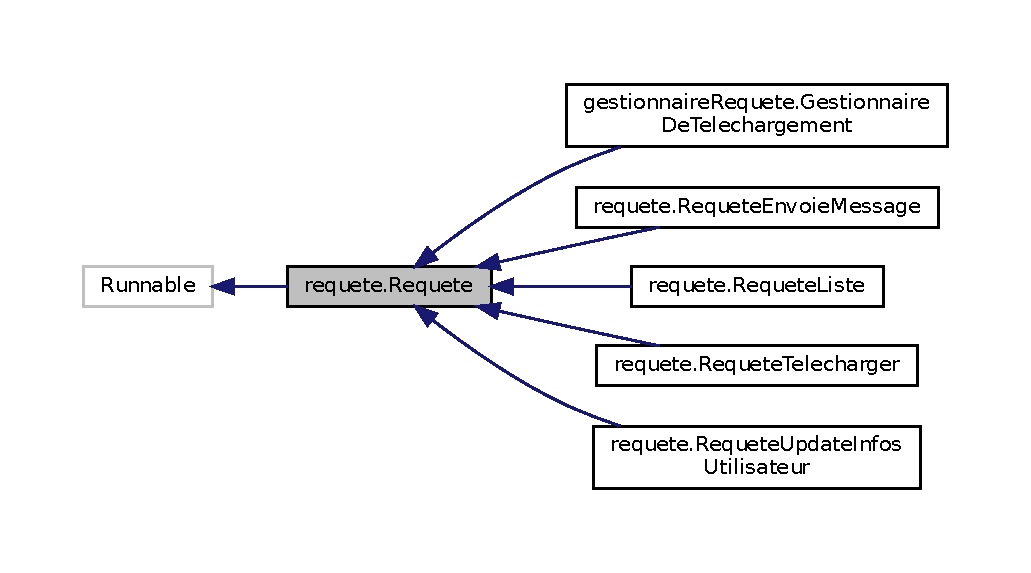
\includegraphics[width=350pt]{classrequete_1_1Requete__inherit__graph}
\end{center}
\end{figure}


Collaboration diagram for requete.\+Requete\+:
\nopagebreak
\begin{figure}[H]
\begin{center}
\leavevmode
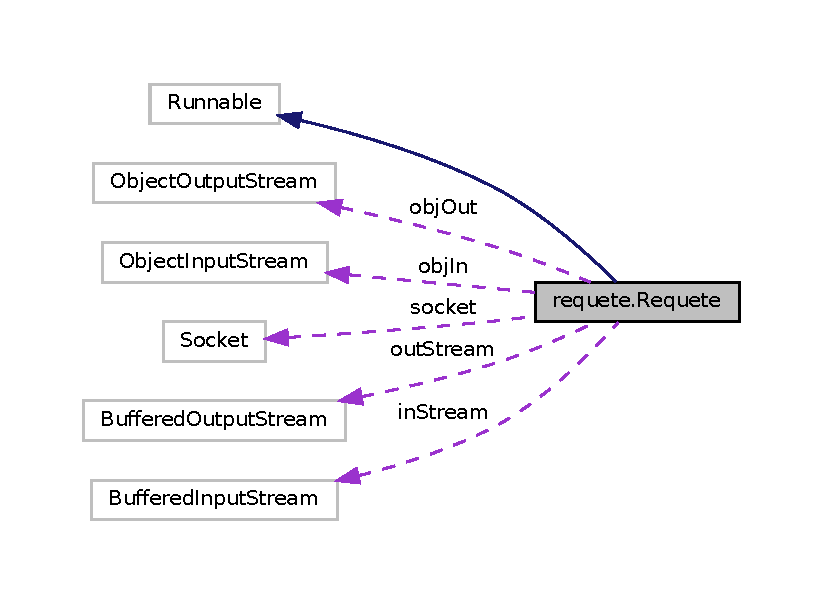
\includegraphics[width=350pt]{classrequete_1_1Requete__coll__graph}
\end{center}
\end{figure}
\subsection*{Public Member Functions}
\begin{DoxyCompactItemize}
\item 
\hyperlink{classrequete_1_1Requete_a6ed8eefb9335b37f2348f5c323a46b53}{Requete} (String adresse\+Serveur)
\begin{DoxyCompactList}\small\item\em constructeur de \hyperlink{classrequete_1_1Requete}{Requete}. \end{DoxyCompactList}\item 
\mbox{\Hypertarget{classrequete_1_1Requete_a919081397ea25302286d7077e3ece323}\label{classrequete_1_1Requete_a919081397ea25302286d7077e3ece323}} 
void \hyperlink{classrequete_1_1Requete_a919081397ea25302286d7077e3ece323}{run} ()
\begin{DoxyCompactList}\small\item\em methode pour lancer le thread. \end{DoxyCompactList}\end{DoxyCompactItemize}
\subsection*{Protected Member Functions}
\begin{DoxyCompactItemize}
\item 
void \hyperlink{classrequete_1_1Requete_a4adc60edaa26be2f8d9b4e4b0a1377cd}{envoyer\+Requete} (String requete)
\begin{DoxyCompactList}\small\item\em envoie une requête au serveur. \end{DoxyCompactList}\item 
\mbox{\Hypertarget{classrequete_1_1Requete_a139183d42763866d351b3569c858b169}\label{classrequete_1_1Requete_a139183d42763866d351b3569c858b169}} 
void \hyperlink{classrequete_1_1Requete_a139183d42763866d351b3569c858b169}{terminer} ()
\begin{DoxyCompactList}\small\item\em fermer les differents éléments du Thread. \end{DoxyCompactList}\end{DoxyCompactItemize}
\subsection*{Protected Attributes}
\begin{DoxyCompactItemize}
\item 
\mbox{\Hypertarget{classrequete_1_1Requete_ac459a04e0e05713cf40d2810141730f1}\label{classrequete_1_1Requete_ac459a04e0e05713cf40d2810141730f1}} 
String {\bfseries ip\+Serveur}
\item 
\mbox{\Hypertarget{classrequete_1_1Requete_a09be09377c9ce1174e027c9bc852c0ab}\label{classrequete_1_1Requete_a09be09377c9ce1174e027c9bc852c0ab}} 
int {\bfseries port\+Serveur}
\item 
\mbox{\Hypertarget{classrequete_1_1Requete_a487b0b95bcb22cd79e17b8ba2756daa6}\label{classrequete_1_1Requete_a487b0b95bcb22cd79e17b8ba2756daa6}} 
Buffered\+Input\+Stream {\bfseries in\+Stream}
\item 
\mbox{\Hypertarget{classrequete_1_1Requete_aec10f73f1c9edcba8a6aeffbd9dc932b}\label{classrequete_1_1Requete_aec10f73f1c9edcba8a6aeffbd9dc932b}} 
Buffered\+Output\+Stream {\bfseries out\+Stream}
\item 
\mbox{\Hypertarget{classrequete_1_1Requete_a8bbfc163d41bdf7d3ed614e0341a1bc8}\label{classrequete_1_1Requete_a8bbfc163d41bdf7d3ed614e0341a1bc8}} 
Socket {\bfseries socket}
\end{DoxyCompactItemize}


\subsection{Detailed Description}
classe abstraite définissant une requête d\textquotesingle{}un client au serveur. 

\subsection{Constructor \& Destructor Documentation}
\mbox{\Hypertarget{classrequete_1_1Requete_a6ed8eefb9335b37f2348f5c323a46b53}\label{classrequete_1_1Requete_a6ed8eefb9335b37f2348f5c323a46b53}} 
\index{requete\+::\+Requete@{requete\+::\+Requete}!Requete@{Requete}}
\index{Requete@{Requete}!requete\+::\+Requete@{requete\+::\+Requete}}
\subsubsection{\texorpdfstring{Requete()}{Requete()}}
{\footnotesize\ttfamily requete.\+Requete.\+Requete (\begin{DoxyParamCaption}\item[{String}]{adresse\+Serveur }\end{DoxyParamCaption})\hspace{0.3cm}{\ttfamily [inline]}}



constructeur de \hyperlink{classrequete_1_1Requete}{Requete}. 


\begin{DoxyParams}{Parameters}
{\em adresse\+Serveur} & adresse et port du serveur de la forme \char`\"{}\+I\+P\+:\+P\+O\+R\+T\char`\"{}. \\
\hline
\end{DoxyParams}


\subsection{Member Function Documentation}
\mbox{\Hypertarget{classrequete_1_1Requete_a4adc60edaa26be2f8d9b4e4b0a1377cd}\label{classrequete_1_1Requete_a4adc60edaa26be2f8d9b4e4b0a1377cd}} 
\index{requete\+::\+Requete@{requete\+::\+Requete}!envoyer\+Requete@{envoyer\+Requete}}
\index{envoyer\+Requete@{envoyer\+Requete}!requete\+::\+Requete@{requete\+::\+Requete}}
\subsubsection{\texorpdfstring{envoyer\+Requete()}{envoyerRequete()}}
{\footnotesize\ttfamily void requete.\+Requete.\+envoyer\+Requete (\begin{DoxyParamCaption}\item[{String}]{requete }\end{DoxyParamCaption})\hspace{0.3cm}{\ttfamily [inline]}, {\ttfamily [protected]}}



envoie une requête au serveur. 


\begin{DoxyParams}{Parameters}
{\em requete} & requete envoyé au serveur. \\
\hline
\end{DoxyParams}


The documentation for this class was generated from the following file\+:\begin{DoxyCompactItemize}
\item 
Requete.\+java\end{DoxyCompactItemize}

\hypertarget{classrequete_1_1RequeteListe}{}\section{requete.\+Requete\+Liste Class Reference}
\label{classrequete_1_1RequeteListe}\index{requete.\+Requete\+Liste@{requete.\+Requete\+Liste}}


Cette classe permet de créer un Thread qui va demander à un serveur la liste des fichiers qu\textquotesingle{}il contient.  




Inheritance diagram for requete.\+Requete\+Liste\+:
% FIG 0


Collaboration diagram for requete.\+Requete\+Liste\+:
% FIG 1
\subsection*{Public Member Functions}
\begin{DoxyCompactItemize}
\item 
\hyperlink{classrequete_1_1RequeteListe_abf11f2cbe8b9eb9eae7621dff966ebd5}{Requete\+Liste} (String adresse\+Serveur)
\begin{DoxyCompactList}\small\item\em constructeur de la classe \hyperlink{classrequete_1_1RequeteListe}{Requete\+Liste} \end{DoxyCompactList}\item 
\mbox{\Hypertarget{classrequete_1_1RequeteListe_a744397e5813266c362903f65965e0e4e}\label{classrequete_1_1RequeteListe_a744397e5813266c362903f65965e0e4e}} 
void \hyperlink{classrequete_1_1RequeteListe_a744397e5813266c362903f65965e0e4e}{run} ()
\begin{DoxyCompactList}\small\item\em methode pour lancer le Thread. \end{DoxyCompactList}\end{DoxyCompactItemize}
\subsection*{Additional Inherited Members}


\subsection{Detailed Description}
Cette classe permet de créer un Thread qui va demander à un serveur la liste des fichiers qu\textquotesingle{}il contient. 

\subsection{Constructor \& Destructor Documentation}
\mbox{\Hypertarget{classrequete_1_1RequeteListe_abf11f2cbe8b9eb9eae7621dff966ebd5}\label{classrequete_1_1RequeteListe_abf11f2cbe8b9eb9eae7621dff966ebd5}} 
\index{requete\+::\+Requete\+Liste@{requete\+::\+Requete\+Liste}!Requete\+Liste@{Requete\+Liste}}
\index{Requete\+Liste@{Requete\+Liste}!requete\+::\+Requete\+Liste@{requete\+::\+Requete\+Liste}}
\subsubsection{\texorpdfstring{Requete\+Liste()}{RequeteListe()}}
{\footnotesize\ttfamily requete.\+Requete\+Liste.\+Requete\+Liste (\begin{DoxyParamCaption}\item[{String}]{adresse\+Serveur }\end{DoxyParamCaption})\hspace{0.3cm}{\ttfamily [inline]}}



constructeur de la classe \hyperlink{classrequete_1_1RequeteListe}{Requete\+Liste} 


\begin{DoxyParams}{Parameters}
{\em adresse\+Serveur} & adresse et port du serveur de la forme \char`\"{}\+I\+P\+:\+P\+O\+R\+T\char`\"{}. \\
\hline
\end{DoxyParams}


The documentation for this class was generated from the following file\+:\begin{DoxyCompactItemize}
\item 
Requete\+Liste.\+java\end{DoxyCompactItemize}

\hypertarget{classrequete_1_1RequeteTelecharger}{}\section{requete.\+Requete\+Telecharger Class Reference}
\label{classrequete_1_1RequeteTelecharger}\index{requete.\+Requete\+Telecharger@{requete.\+Requete\+Telecharger}}


cette classe va télécharger un bloc de fichier depuis un serveur.  




Inheritance diagram for requete.\+Requete\+Telecharger\+:\nopagebreak
\begin{figure}[H]
\begin{center}
\leavevmode
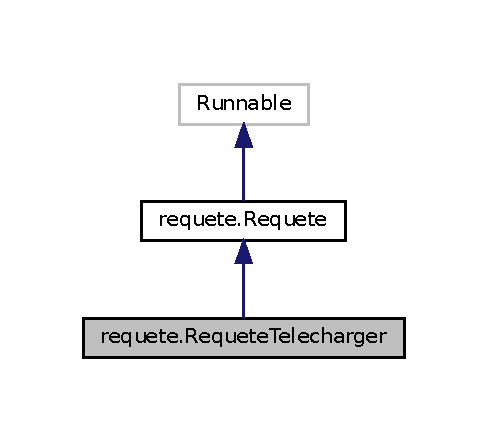
\includegraphics[width=220pt]{classrequete_1_1RequeteTelecharger__inherit__graph}
\end{center}
\end{figure}


Collaboration diagram for requete.\+Requete\+Telecharger\+:\nopagebreak
\begin{figure}[H]
\begin{center}
\leavevmode
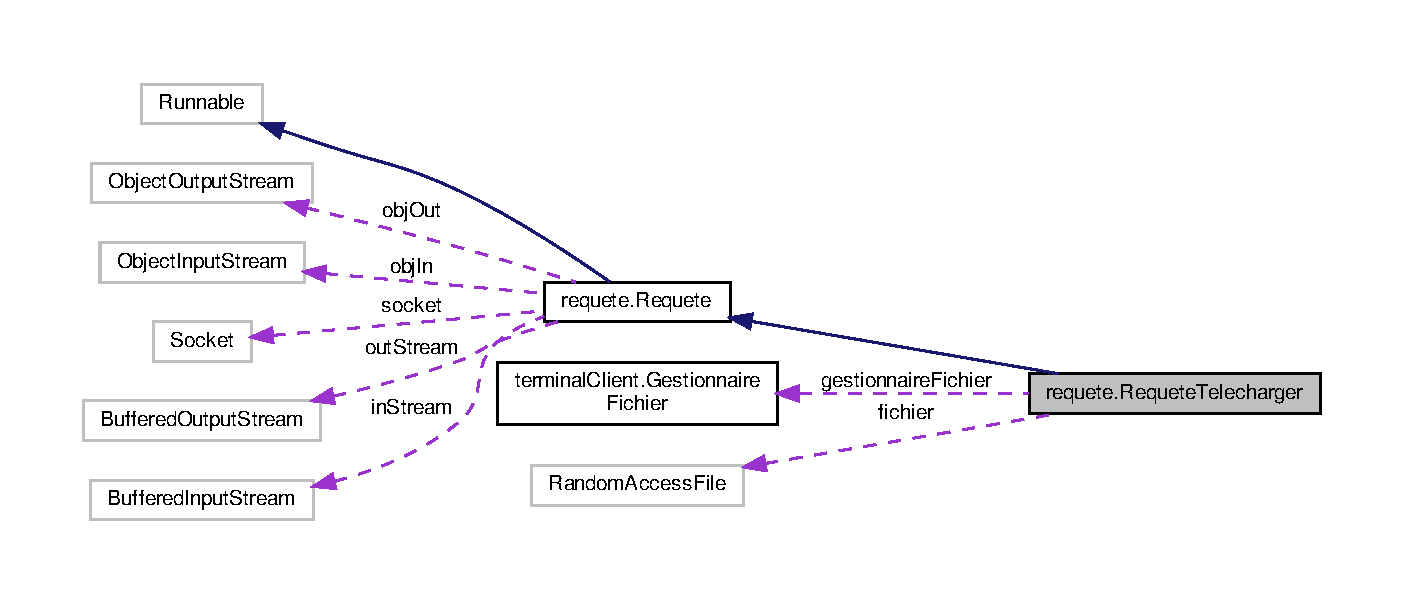
\includegraphics[width=350pt]{classrequete_1_1RequeteTelecharger__coll__graph}
\end{center}
\end{figure}
\subsection*{Public Member Functions}
\begin{DoxyCompactItemize}
\item 
\hyperlink{classrequete_1_1RequeteTelecharger_a5c4fa1ef19064d12dc2ed51ecc5f3ba3}{Requete\+Telecharger} (String adresse\+Serveur, Random\+Access\+File fichier, String nom\+Fichier, \hyperlink{classterminalClient_1_1GestionnaireFichier}{Gestionnaire\+Fichier} gestionnaire\+Fichier, int numero\+Du\+Bloc)
\begin{DoxyCompactList}\small\item\em constructeur de la classe permettant de télécharger une bloc d\textquotesingle{}un fichier depuis un serveur. \end{DoxyCompactList}\item 
\mbox{\Hypertarget{classrequete_1_1RequeteTelecharger_a89314ecc5cdf732dd3f1d670dc13551f}\label{classrequete_1_1RequeteTelecharger_a89314ecc5cdf732dd3f1d670dc13551f}} 
void \hyperlink{classrequete_1_1RequeteTelecharger_a89314ecc5cdf732dd3f1d670dc13551f}{run} ()
\begin{DoxyCompactList}\small\item\em methode pour lancer le Thread. \end{DoxyCompactList}\end{DoxyCompactItemize}
\subsection*{Additional Inherited Members}


\subsection{Detailed Description}
cette classe va télécharger un bloc de fichier depuis un serveur. 

\subsection{Constructor \& Destructor Documentation}
\mbox{\Hypertarget{classrequete_1_1RequeteTelecharger_a5c4fa1ef19064d12dc2ed51ecc5f3ba3}\label{classrequete_1_1RequeteTelecharger_a5c4fa1ef19064d12dc2ed51ecc5f3ba3}} 
\index{requete\+::\+Requete\+Telecharger@{requete\+::\+Requete\+Telecharger}!Requete\+Telecharger@{Requete\+Telecharger}}
\index{Requete\+Telecharger@{Requete\+Telecharger}!requete\+::\+Requete\+Telecharger@{requete\+::\+Requete\+Telecharger}}
\subsubsection{\texorpdfstring{Requete\+Telecharger()}{RequeteTelecharger()}}
{\footnotesize\ttfamily requete.\+Requete\+Telecharger.\+Requete\+Telecharger (\begin{DoxyParamCaption}\item[{String}]{adresse\+Serveur,  }\item[{Random\+Access\+File}]{fichier,  }\item[{String}]{nom\+Fichier,  }\item[{\hyperlink{classterminalClient_1_1GestionnaireFichier}{Gestionnaire\+Fichier}}]{gestionnaire\+Fichier,  }\item[{int}]{numero\+Du\+Bloc }\end{DoxyParamCaption})\hspace{0.3cm}{\ttfamily [inline]}}



constructeur de la classe permettant de télécharger une bloc d\textquotesingle{}un fichier depuis un serveur. 


\begin{DoxyParams}{Parameters}
{\em adresse\+Serveur} & adresse du serveur et son port en format $<$\+I\+P$>$\+:$<$\+P\+O\+R\+T$>$. \\
\hline
{\em nom\+Fichier} & nom du fichier à télécharger. \\
\hline
{\em gestionnaire\+Fichier} & le gestionnaire de fichier. \\
\hline
{\em numero\+Du\+Bloc} & numéro du bloc du fichier que l\textquotesingle{}on souhaite télécharger. \\
\hline
\end{DoxyParams}


The documentation for this class was generated from the following file\+:\begin{DoxyCompactItemize}
\item 
Requete\+Telecharger.\+java\end{DoxyCompactItemize}

\hypertarget{classrequete_1_1RequeteUpdateInfosUtilisateur}{}\section{requete.\+Requete\+Update\+Infos\+Utilisateur Class Reference}
\label{classrequete_1_1RequeteUpdateInfosUtilisateur}\index{requete.\+Requete\+Update\+Infos\+Utilisateur@{requete.\+Requete\+Update\+Infos\+Utilisateur}}


cette classe permet d\textquotesingle{}envoyer au serveur central les infos concernant le client.  




Inheritance diagram for requete.\+Requete\+Update\+Infos\+Utilisateur\+:\nopagebreak
\begin{figure}[H]
\begin{center}
\leavevmode
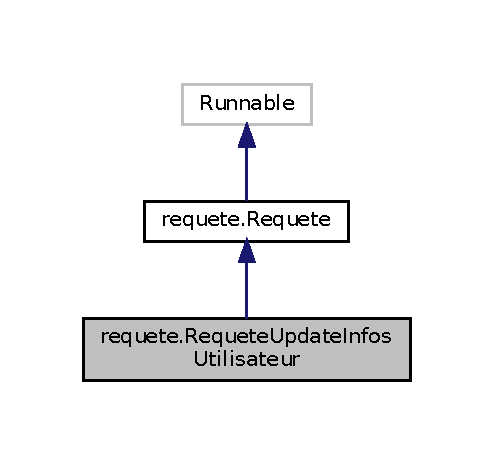
\includegraphics[width=222pt]{classrequete_1_1RequeteUpdateInfosUtilisateur__inherit__graph}
\end{center}
\end{figure}


Collaboration diagram for requete.\+Requete\+Update\+Infos\+Utilisateur\+:\nopagebreak
\begin{figure}[H]
\begin{center}
\leavevmode
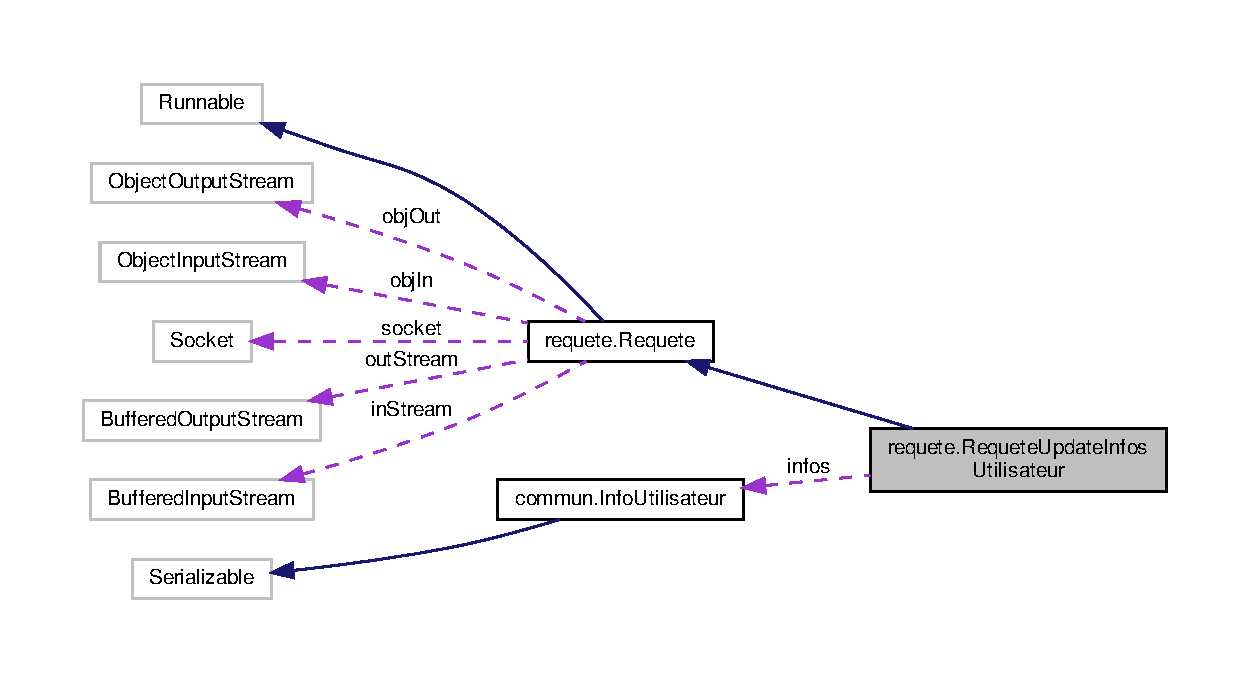
\includegraphics[width=350pt]{classrequete_1_1RequeteUpdateInfosUtilisateur__coll__graph}
\end{center}
\end{figure}
\subsection*{Public Member Functions}
\begin{DoxyCompactItemize}
\item 
\hyperlink{classrequete_1_1RequeteUpdateInfosUtilisateur_af4ad8be6ca59ea30a643d98b44fd6b82}{Requete\+Update\+Infos\+Utilisateur} (String adresse\+Serveur\+Central, \hyperlink{classcommun_1_1InfoUtilisateur}{Info\+Utilisateur} infos)
\begin{DoxyCompactList}\small\item\em constructeur de la classe. \end{DoxyCompactList}\item 
\mbox{\Hypertarget{classrequete_1_1RequeteUpdateInfosUtilisateur_af28513ad85d93be736ca76bf950fa55b}\label{classrequete_1_1RequeteUpdateInfosUtilisateur_af28513ad85d93be736ca76bf950fa55b}} 
void \hyperlink{classrequete_1_1RequeteUpdateInfosUtilisateur_af28513ad85d93be736ca76bf950fa55b}{run} ()
\begin{DoxyCompactList}\small\item\em méthode pour lancer le Thread. \end{DoxyCompactList}\end{DoxyCompactItemize}
\subsection*{Additional Inherited Members}


\subsection{Detailed Description}
cette classe permet d\textquotesingle{}envoyer au serveur central les infos concernant le client. 

\subsection{Constructor \& Destructor Documentation}
\mbox{\Hypertarget{classrequete_1_1RequeteUpdateInfosUtilisateur_af4ad8be6ca59ea30a643d98b44fd6b82}\label{classrequete_1_1RequeteUpdateInfosUtilisateur_af4ad8be6ca59ea30a643d98b44fd6b82}} 
\index{requete\+::\+Requete\+Update\+Infos\+Utilisateur@{requete\+::\+Requete\+Update\+Infos\+Utilisateur}!Requete\+Update\+Infos\+Utilisateur@{Requete\+Update\+Infos\+Utilisateur}}
\index{Requete\+Update\+Infos\+Utilisateur@{Requete\+Update\+Infos\+Utilisateur}!requete\+::\+Requete\+Update\+Infos\+Utilisateur@{requete\+::\+Requete\+Update\+Infos\+Utilisateur}}
\subsubsection{\texorpdfstring{Requete\+Update\+Infos\+Utilisateur()}{RequeteUpdateInfosUtilisateur()}}
{\footnotesize\ttfamily requete.\+Requete\+Update\+Infos\+Utilisateur.\+Requete\+Update\+Infos\+Utilisateur (\begin{DoxyParamCaption}\item[{String}]{adresse\+Serveur\+Central,  }\item[{\hyperlink{classcommun_1_1InfoUtilisateur}{Info\+Utilisateur}}]{infos }\end{DoxyParamCaption})\hspace{0.3cm}{\ttfamily [inline]}}



constructeur de la classe. 


\begin{DoxyParams}{Parameters}
{\em adresse\+Serveur} & l\textquotesingle{}adresse du serveur central, format $<$\+I\+P$>$\+:$<$\+P\+O\+R\+T$>$ . \\
\hline
{\em infos} & les infos de l\textquotesingle{}utilisateur à envoyer au serveur central. \\
\hline
\end{DoxyParams}


The documentation for this class was generated from the following file\+:\begin{DoxyCompactItemize}
\item 
Requete\+Update\+Infos\+Utilisateur.\+java\end{DoxyCompactItemize}

\hypertarget{classterminalClient_1_1Serveur}{}\section{terminal\+Client.\+Serveur Class Reference}
\label{classterminalClient_1_1Serveur}\index{terminal\+Client.\+Serveur@{terminal\+Client.\+Serveur}}


Cette classe gère les fonctionnalitées de serveur d\textquotesingle{}un client.  




Inheritance diagram for terminal\+Client.\+Serveur\+:\nopagebreak
\begin{figure}[H]
\begin{center}
\leavevmode
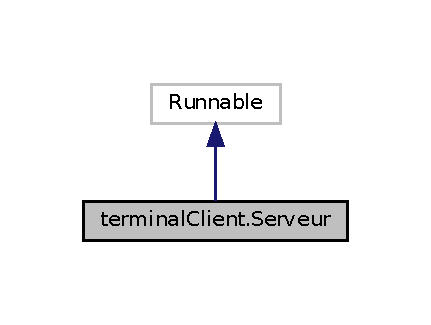
\includegraphics[width=193pt]{classterminalClient_1_1Serveur__inherit__graph}
\end{center}
\end{figure}


Collaboration diagram for terminal\+Client.\+Serveur\+:\nopagebreak
\begin{figure}[H]
\begin{center}
\leavevmode
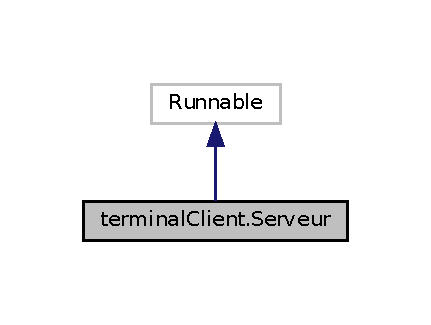
\includegraphics[width=193pt]{classterminalClient_1_1Serveur__coll__graph}
\end{center}
\end{figure}
\subsection*{Public Member Functions}
\begin{DoxyCompactItemize}
\item 
\hyperlink{classterminalClient_1_1Serveur_afb46fedaf8b4dd05eac7f7931a8587dd}{Serveur} (int port, \hyperlink{classterminalClient_1_1GestionnaireFichier}{Gestionnaire\+Fichier} gestionnaire\+De\+Fichier, String ip\+Serveur\+Central, int port\+Serveur\+Central)
\begin{DoxyCompactList}\small\item\em constructeur de la classe \end{DoxyCompactList}\item 
void \hyperlink{classterminalClient_1_1Serveur_a3231a51ed25972d4b52e7aed302efea5}{run} ()
\begin{DoxyCompactList}\small\item\em méthode pour lancer le Thread. \end{DoxyCompactList}\end{DoxyCompactItemize}


\subsection{Detailed Description}
Cette classe gère les fonctionnalitées de serveur d\textquotesingle{}un client. 

\subsection{Constructor \& Destructor Documentation}
\mbox{\Hypertarget{classterminalClient_1_1Serveur_afb46fedaf8b4dd05eac7f7931a8587dd}\label{classterminalClient_1_1Serveur_afb46fedaf8b4dd05eac7f7931a8587dd}} 
\index{terminal\+Client\+::\+Serveur@{terminal\+Client\+::\+Serveur}!Serveur@{Serveur}}
\index{Serveur@{Serveur}!terminal\+Client\+::\+Serveur@{terminal\+Client\+::\+Serveur}}
\subsubsection{\texorpdfstring{Serveur()}{Serveur()}}
{\footnotesize\ttfamily terminal\+Client.\+Serveur.\+Serveur (\begin{DoxyParamCaption}\item[{int}]{port,  }\item[{\hyperlink{classterminalClient_1_1GestionnaireFichier}{Gestionnaire\+Fichier}}]{gestionnaire\+De\+Fichier,  }\item[{String}]{ip\+Serveur\+Central,  }\item[{int}]{port\+Serveur\+Central }\end{DoxyParamCaption})\hspace{0.3cm}{\ttfamily [inline]}}



constructeur de la classe 


\begin{DoxyParams}{Parameters}
{\em port} & le port d\textquotesingle{}écoute de la fonctionnalité serveur du client. \\
\hline
{\em gestionnaire\+De\+Fichier} & le gestionnaire de fichier. \\
\hline
{\em ip\+Serveur\+Central} & l\textquotesingle{}ip du serveur central. \\
\hline
{\em port\+Serveur\+Central} & le port du serveur central. \\
\hline
\end{DoxyParams}


\subsection{Member Function Documentation}
\mbox{\Hypertarget{classterminalClient_1_1Serveur_a3231a51ed25972d4b52e7aed302efea5}\label{classterminalClient_1_1Serveur_a3231a51ed25972d4b52e7aed302efea5}} 
\index{terminal\+Client\+::\+Serveur@{terminal\+Client\+::\+Serveur}!run@{run}}
\index{run@{run}!terminal\+Client\+::\+Serveur@{terminal\+Client\+::\+Serveur}}
\subsubsection{\texorpdfstring{run()}{run()}}
{\footnotesize\ttfamily void terminal\+Client.\+Serveur.\+run (\begin{DoxyParamCaption}{ }\end{DoxyParamCaption})\hspace{0.3cm}{\ttfamily [inline]}}



méthode pour lancer le Thread. 

cette méthode lance le serveur en ouvrant la socket de rendez-\/vous, la méthode va par la suite attendre la venue d\textquotesingle{}un client puis transferer chaque connexion au gestionnaire de client pour qu\textquotesingle{}il traite les requête de chaque client dans un Thread unique. 

The documentation for this class was generated from the following file\+:\begin{DoxyCompactItemize}
\item 
Serveur.\+java\end{DoxyCompactItemize}

\hypertarget{classcentralServer_1_1ServeurCentral}{}\section{central\+Server.\+Serveur\+Central Class Reference}
\label{classcentralServer_1_1ServeurCentral}\index{central\+Server.\+Serveur\+Central@{central\+Server.\+Serveur\+Central}}
\subsection*{Public Member Functions}
\begin{DoxyCompactItemize}
\item 
\hyperlink{classcentralServer_1_1ServeurCentral_a0a086fea144fda9d64564199aa9de857}{Serveur\+Central} (int port)
\begin{DoxyCompactList}\small\item\em constructeur de \hyperlink{classcentralServer_1_1ServeurCentral}{Serveur\+Central} \end{DoxyCompactList}\item 
\mbox{\Hypertarget{classcentralServer_1_1ServeurCentral_a48440e395e1ad3a3c4eca13ca4245bd5}\label{classcentralServer_1_1ServeurCentral_a48440e395e1ad3a3c4eca13ca4245bd5}} 
void {\bfseries lancer} ()
\end{DoxyCompactItemize}


\subsection{Constructor \& Destructor Documentation}
\mbox{\Hypertarget{classcentralServer_1_1ServeurCentral_a0a086fea144fda9d64564199aa9de857}\label{classcentralServer_1_1ServeurCentral_a0a086fea144fda9d64564199aa9de857}} 
\index{central\+Server\+::\+Serveur\+Central@{central\+Server\+::\+Serveur\+Central}!Serveur\+Central@{Serveur\+Central}}
\index{Serveur\+Central@{Serveur\+Central}!central\+Server\+::\+Serveur\+Central@{central\+Server\+::\+Serveur\+Central}}
\subsubsection{\texorpdfstring{Serveur\+Central()}{ServeurCentral()}}
{\footnotesize\ttfamily central\+Server.\+Serveur\+Central.\+Serveur\+Central (\begin{DoxyParamCaption}\item[{int}]{port }\end{DoxyParamCaption})\hspace{0.3cm}{\ttfamily [inline]}}



constructeur de \hyperlink{classcentralServer_1_1ServeurCentral}{Serveur\+Central} 


\begin{DoxyParams}{Parameters}
{\em port} & port sur lequel va écouter le serveur central. \\
\hline
\end{DoxyParams}


The documentation for this class was generated from the following file\+:\begin{DoxyCompactItemize}
\item 
Serveur\+Central.\+java\end{DoxyCompactItemize}

\hypertarget{classcentralServer_1_1ServeurCentralMain}{}\section{central\+Server.\+Serveur\+Central\+Main Class Reference}
\label{classcentralServer_1_1ServeurCentralMain}\index{central\+Server.\+Serveur\+Central\+Main@{central\+Server.\+Serveur\+Central\+Main}}
\subsection*{Static Public Member Functions}
\begin{DoxyCompactItemize}
\item 
\mbox{\Hypertarget{classcentralServer_1_1ServeurCentralMain_a4a243b7e767f8cda08f3d9793182bbf9}\label{classcentralServer_1_1ServeurCentralMain_a4a243b7e767f8cda08f3d9793182bbf9}} 
static void {\bfseries main} (String\mbox{[}$\,$\mbox{]} args)
\end{DoxyCompactItemize}


The documentation for this class was generated from the following file\+:\begin{DoxyCompactItemize}
\item 
Serveur\+Central\+Main.\+java\end{DoxyCompactItemize}

\hypertarget{classterminalClient_1_1TerminalMain}{}\section{terminal\+Client.\+Terminal\+Main Class Reference}
\label{classterminalClient_1_1TerminalMain}\index{terminal\+Client.\+Terminal\+Main@{terminal\+Client.\+Terminal\+Main}}
\subsection*{Static Public Member Functions}
\begin{DoxyCompactItemize}
\item 
\mbox{\Hypertarget{classterminalClient_1_1TerminalMain_a8152b318f8e64093d4da2e08b1628056}\label{classterminalClient_1_1TerminalMain_a8152b318f8e64093d4da2e08b1628056}} 
static void {\bfseries main} (String\mbox{[}$\,$\mbox{]} args)
\end{DoxyCompactItemize}


The documentation for this class was generated from the following file\+:\begin{DoxyCompactItemize}
\item 
Terminal\+Main.\+java\end{DoxyCompactItemize}

%--- End generated contents ---

% Index
\backmatter
\newpage
\phantomsection
\clearemptydoublepage
\addcontentsline{toc}{chapter}{Index}
\printindex

\end{document}
